%% COMPILE WITH XeLaTeX %%
\documentclass[svgnames,oneside,openright,a4paper,10pt]{book}
\usepackage{tikz,booktabs}
\usepackage[danish]{babel}
\usepackage[lf]{venturis}
\usepackage[explicit]{titlesec}
\usepackage[sort&compress]{natbib}
\renewcommand*\familydefault{\sfdefault}
\usepackage{fontspec}
\setmainfont{Arial}
%\setsecfont{Neo Tech Std}
%\usepackage[T1]{fontenc}
\usepackage[applemac]{inputenc}
\usepackage[colorlinks]{hyperref}
\usepackage{graphicx}
\bibliographystyle{astron}
\usepackage{fancyhdr}
\usepackage{varioref,caption,subcaption}
\usepackage[draft,inline]{fixme}
\usepackage{appendix}
\usepackage{amsmath, latexsym}
\usepackage[notref,notcite,draft]{showkeys}
\usepackage[a4paper]{geometry}
\usepackage{multirow}
\parindent 0pt

\definecolor{DDS}{cmyk}{1,.7,0,.3}
% ------------------------ Header setup  ------------------------ %
\newcommand{\fncyfront}{%
	\fancyhead [RO] {{\footnotesize \rightmark}}
	\fancyfoot [RO] {\thepage}
	\fancyhead [LE] {{\footnotesize \leftmark}}
	\fancyfoot [LE] {\thepage}
	\fancyhead [RE,LO] {}
	\fancyfoot [C] {}
	\renewcommand{\headrulewidth}{0.3pt}}	
\newcommand{\fncymain}{%
	\fancyhead [RO] {{\footnotesize \rightmark}}
	\fancyfoot [RO] {\thepage} 
	\fancyhead [LE] {{\footnotesize \leftmark}}
	\fancyfoot [LE] {\thepage}
	\fancyfoot [C] {}
	\renewcommand{\headrulewidth}{0.3pt}}		
\newcommand{\fncyappendix}{%
	\fancyhead [RO] {{\footnotesize \rightmark}}
	\fancyfoot [RO] {\thepage}
	\fancyhead [LE] {{\footnotesize \leftmark}}
	\fancyfoot [LE] {\thepage}
	\fancyhead [RE,LO] {}
	\fancyfoot [C] {}	
	\renewcommand{\headrulewidth}{0.3pt}
	\renewcommand{\footrulewidth}{0.3pt}}
\makeatletter
\def\cleardoublepage{\clearpage\if@twoside
\ifodd\c@page
\else\hbox{}\thispagestyle{empty}\newpage
\if@twocolumn\hbox{}\newpage\fi\fi\fi}
\makeatother 
\pagestyle{fancy}

%%%%%%%%%%%%%%%%%%%%%%%%%%%%%%%%%%%%%%%%%	 Bibliography 		%%%%%%%%%%%%%%%%%%%%%%%%%%%%%%%%%%%%%%%%%%%%%%%%%%%%
\def\aj{AJ}%
          % Astronomical Journal
\def\actaa{Acta Astron.}%
          % Acta Astronomica
\def\araa{ARA\&A}%
          % Annual Review of Astron and Astrophys
\def\apj{ApJ}%
          % Astrophysical Journal
\def\apjl{ApJ}%
          % Astrophysical Journal, Letters
\def\apjs{ApJS}%
          % Astrophysical Journal, Supplement
\def\ao{Appl.~Opt.}%
          % Applied Optics
\def\apss{Ap\&SS}%
          % Astrophysics and Space Science
\def\aap{A\&A}%
          % Astronomy and Astrophysics
\def\aapr{A\&A~Rev.}%
          % Astronomy and Astrophysics Reviews
\def\aaps{A\&AS}%
          % Astronomy and Astrophysics, Supplement
\def\azh{AZh}%
          % Astronomicheskii Zhurnal
\def\baas{BAAS}%
          % Bulletin of the AAS
\def\bac{Bull. astr. Inst. Czechosl.}%
          % Bulletin of the Astronomical Institutes of Czechoslovakia 
\def\caa{Chinese Astron. Astrophys.}%
          % Chinese Astronomy and Astrophysics
\def\cjaa{Chinese J. Astron. Astrophys.}%
          % Chinese Journal of Astronomy and Astrophysics
\def\icarus{Icarus}%
          % Icarus
\def\jcap{J. Cosmology Astropart. Phys.}%
          % Journal of Cosmology and Astroparticle Physics
\def\jrasc{JRASC}%
          % Journal of the RAS of Canada
\def\mnras{MNRAS}%
          % Monthly Notices of the RAS
\def\memras{MmRAS}%
          % Memoirs of the RAS
\def\na{New A}%
          % New Astronomy
\def\nar{New A Rev.}%
          % New Astronomy Review
\def\pasa{PASA}%
          % Publications of the Astron. Soc. of Australia
\def\pra{Phys.~Rev.~A}%
          % Physical Review A: General Physics
\def\prb{Phys.~Rev.~B}%
          % Physical Review B: Solid State
\def\prc{Phys.~Rev.~C}%
          % Physical Review C
\def\prd{Phys.~Rev.~D}%
          % Physical Review D
\def\pre{Phys.~Rev.~E}%
          % Physical Review E
\def\prl{Phys.~Rev.~Lett.}%
          % Physical Review Letters
\def\pasp{PASP}%
          % Publications of the ASP
\def\pasj{PASJ}%
          % Publications of the ASJ
\def\qjras{QJRAS}%
          % Quarterly Journal of the RAS
\def\rmxaa{Rev. Mexicana Astron. Astrofis.}%
          % Revista Mexicana de Astronomia y Astrofisica
\def\skytel{S\&T}%
          % Sky and Telescope
\def\solphys{Sol.~Phys.}%
          % Solar Physics
\def\sovast{Soviet~Ast.}%
          % Soviet Astronomy
\def\ssr{Space~Sci.~Rev.}%
          % Space Science Reviews
\def\zap{ZAp}%
          % Zeitschrift fuer Astrophysik
\def\nat{Nature}%
          % Nature
\def\iaucirc{IAU~Circ.}%
          % IAU Cirulars
\def\aplett{Astrophys.~Lett.}%
          % Astrophysics Letters
\def\apspr{Astrophys.~Space~Phys.~Res.}%
          % Astrophysics Space Physics Research
\def\bain{Bull.~Astron.~Inst.~Netherlands}%
          % Bulletin Astronomical Institute of the Netherlands
\def\fcp{Fund.~Cosmic~Phys.}%
          % Fundamental Cosmic Physics
\def\gca{Geochim.~Cosmochim.~Acta}%
          % Geochimica Cosmochimica Acta
\def\grl{Geophys.~Res.~Lett.}%
          % Geophysics Research Letters
\def\jcp{J.~Chem.~Phys.}%
          % Journal of Chemical Physics
\def\jgr{J.~Geophys.~Res.}%
          % Journal of Geophysics Research
\def\jqsrt{J.~Quant.~Spec.~Radiat.~Transf.}%
          % Journal of Quantitiative Spectroscopy and Radiative Trasfer
\def\memsai{Mem.~Soc.~Astron.~Italiana}%
          % Mem. Societa Astronomica Italiana
\def\nphysa{Nucl.~Phys.~A}%
          % Nuclear Physics A
\def\physrep{Phys.~Rep.}%
          % Physics Reports
\def\physscr{Phys.~Scr}%
          % Physica Scripta
\def\planss{Planet.~Space~Sci.}%
          % Planetary Space Science
\def\procspie{Proc.~SPIE}%
          % Proceedings of the SPIE
\let\astap=\aap
\let\apjlett=\apjl
\let\apjsupp=\apjs
\let\applopt=\ao

% ------------------------ Abstract setup  ------------------------ %
\newenvironment{abstract}%
{\cleardoublepage\null \vfill\begin{center}%
\bfseries \abstractname \end{center}}%
	{\vfill\null}

% ------------------------ Chapter setup  ------------------------ %
\titleformat{\section}[hang]%
	{\color{DDS}\fontspec[SizeFeatures={{Size=14}}]{Neo Tech Std Light}}%
	{\hspace{20pt}\MakeUppercase{\thesection#1 }} %
	{\parindent}%
	{}%
\titleformat{\subsection}[hang]%
	{\color{MGR}\fontspec[SizeFeatures={{Size=12}}]{Neo Tech Std}}%
	{\hspace{20pt}\MakeUppercase{\thesubsection#1 }}%
	{\parindent}%
	{}%	
\newcommand*\chapterlabel{}
\titleformat{\chapter}
	{\gdef\chapterlabel{}
	 }% \normalfont\sffamily\Huge}
	{\gdef\chapterlabel{\thechapter\ }}{0pt}
	{\begin{tikzpicture}[remember picture, overlay]
		\node[yshift=-3cm] at (current page.north west)
			{\begin{tikzpicture} [remember picture, overlay]
				\draw[very thick, fill=DDS,draw=LightSkyBlue] (0,0) rectangle (\paperwidth, 3cm);
				\draw[thick, fill=LightSkyBlue,draw=DDS,anchor=west, xshift=.075\paperwidth, yshift=-.5cm] (0,0) rectangle (.95\paperwidth, 2cm);
				\draw[draw=LightSkyBlue,fill=white,anchor=west,xshift=.925\paperwidth] (0,0) rectangle (.075\paperwidth,3cm);
				%\draw[draw=DDS,fill=DDS,anchor=west,xshift=.925\paperwidth,yshift=.03cm] (0,0) rectangle (.075\paperwidth,2.3cm);
				\draw[draw=LightSkyBlue,fill=LightSkyBlue,anchor=west,xshift=.925\paperwidth,yshift=0cm] (0,0) rectangle (.075\paperwidth,2.3cm);
				\node[anchor=west, xshift=.1\paperwidth,yshift=.55cm,rectangle, fill=LightSkyBlue]%rounded corners=20pt, inner sep=11pt, fill=DDS]
				{\fontspec[SizeFeatures={{Size=24}}]{Neo Tech Std}\color{DDS}\MakeUppercase{\chapterlabel#1}};
			\end{tikzpicture}
			};
		\end{tikzpicture}
	}
	\titlespacing*{\chapter}{0pt}{50pt}{-40pt}
	
% ------------------------ Custom setup  ------------------------ %	
\newcommand{\figref}[1]{figur \ref{fig:#1}}
\newcommand{\tblref}[1]{tabel \ref{tbl:#1}}
\newcommand{\secref}[1]{afsnit \ref{sec:#1}}
\newcommand{\appref}[1]{appendix \ref{app:#1}}
\renewcommand{\eqref}[1]{ligning (\ref{eq:#1})}
\newcommand{\chapref}[1]{kapitel \ref{ch:#1}}
\graphicspath{{figures/}}	

\begin{document}
	%\raggedbottom
	\fncyfront
	\frontmatter
	\input{chapters/frontmatter}
	\input{chapters/forord}
	\tableofcontents
	\listoftables
	\listoffigures

\mainmatter
% ------------------------ Mainmatter setup  ------------------------ %	
%	- Introduktion								 %
%	- Problemformulering						 %
%	- Main									 %
%	- Konklusion								 %
% -------------------------------------------------------------------------- %

\chapter{Introduktion}
\label{ch:Intro}

Denne opgave tager sit udspring i et forl�b om verdensbilleder. Forl�bet verdensbilleder er det f�rste kernestof omr�de i l�rerplanen for alle niveauer i fysik. Denne opgaves forl�b er tilrettet l�rerplanen for fysik B \citet{FysB}. Forl�bet er essentielt da det s�tter faget ind i en historisk kontekst som mange elever finder utrolig sp�ndende. Jeg har oplevet at flere undervisere som ikke finder den videnskabshistoriske del af fysikken lige s� vigtig som de �vrige kernestof omr�der, jeg derimod har med dette forl�b valgt at fokusere s�rligt meget p� elevernes forst�else af fagets udvikling gennem tiden. Dette giver eleverne en god for-forst�else for det efterf�lgende stof.
Forl�bet har v�ret gennemf�rt  i to klasser uafh�ngigt af hinanden. 

\section{~Naturvidenskabelige studieretninger}
\label{sec:NVst}

Den ene klasse var 2. bm som er en klasse med bioteknologi som studieretning. Det betyder at klassen har bioteknologi A, matematik A og fysik B. Fysik forl�bet for klassen starter i 2. g. Klassen er pr�get af at denne studieretning tiltr�kker forholdsvist mange piger som det fremg�r af \tblref{dreng:pige}, markeret med r�d. Den anden klasse som har v�ret m�l for dette forl�b er 1.m som ligeledes er fremh�vet med r�d i \tblref{dreng:pige} denne studieretning tiltr�kker flest drenge. 

\begin{table}[h!]
	\centering
	\caption[K�nsfordeling p� studieretninger]{Tabellen viser k�nsfordelingen p� Marselisborg Gymnasiums naturvidenskabelige studieretninger for �rene 2010/11 - 2012/13, med r�dt er markeret de klasser som har gennemf�rt forl�bet om verdensbilleder.}
	\label{tbl:dreng:pige}
	\begin{tabular}{@{ } l l l l l l l @{ }}
		\toprule[2pt]
		Optagelses	& \multicolumn{2}{c}{Biotek. (bm)}	& \multicolumn{2}{c}{Ma. - Bi. (mb)}	& \multicolumn{2}{c}{Ma. - Fy.- Ke. (m)}\\
		�r			& Piger	& Drenge				& Piger	& Drenge 				& Piger	& Drenge \\
		\midrule[1.2pt]
		2010/11		& 16		& 11					& 13		& 15					& 9		& 16\\
		2011/12		& {\color{red}21}		& {\color{red}9}					& 13		& 15					& 7		& 21\\
		2012/13		&12		& 10					& 7		& 22					& {\color{red}8}		& {\color{red}20}\\
		\bottomrule[2pt]
	\end{tabular}
\end{table}

\begin{figure}[h!]
	\centering
	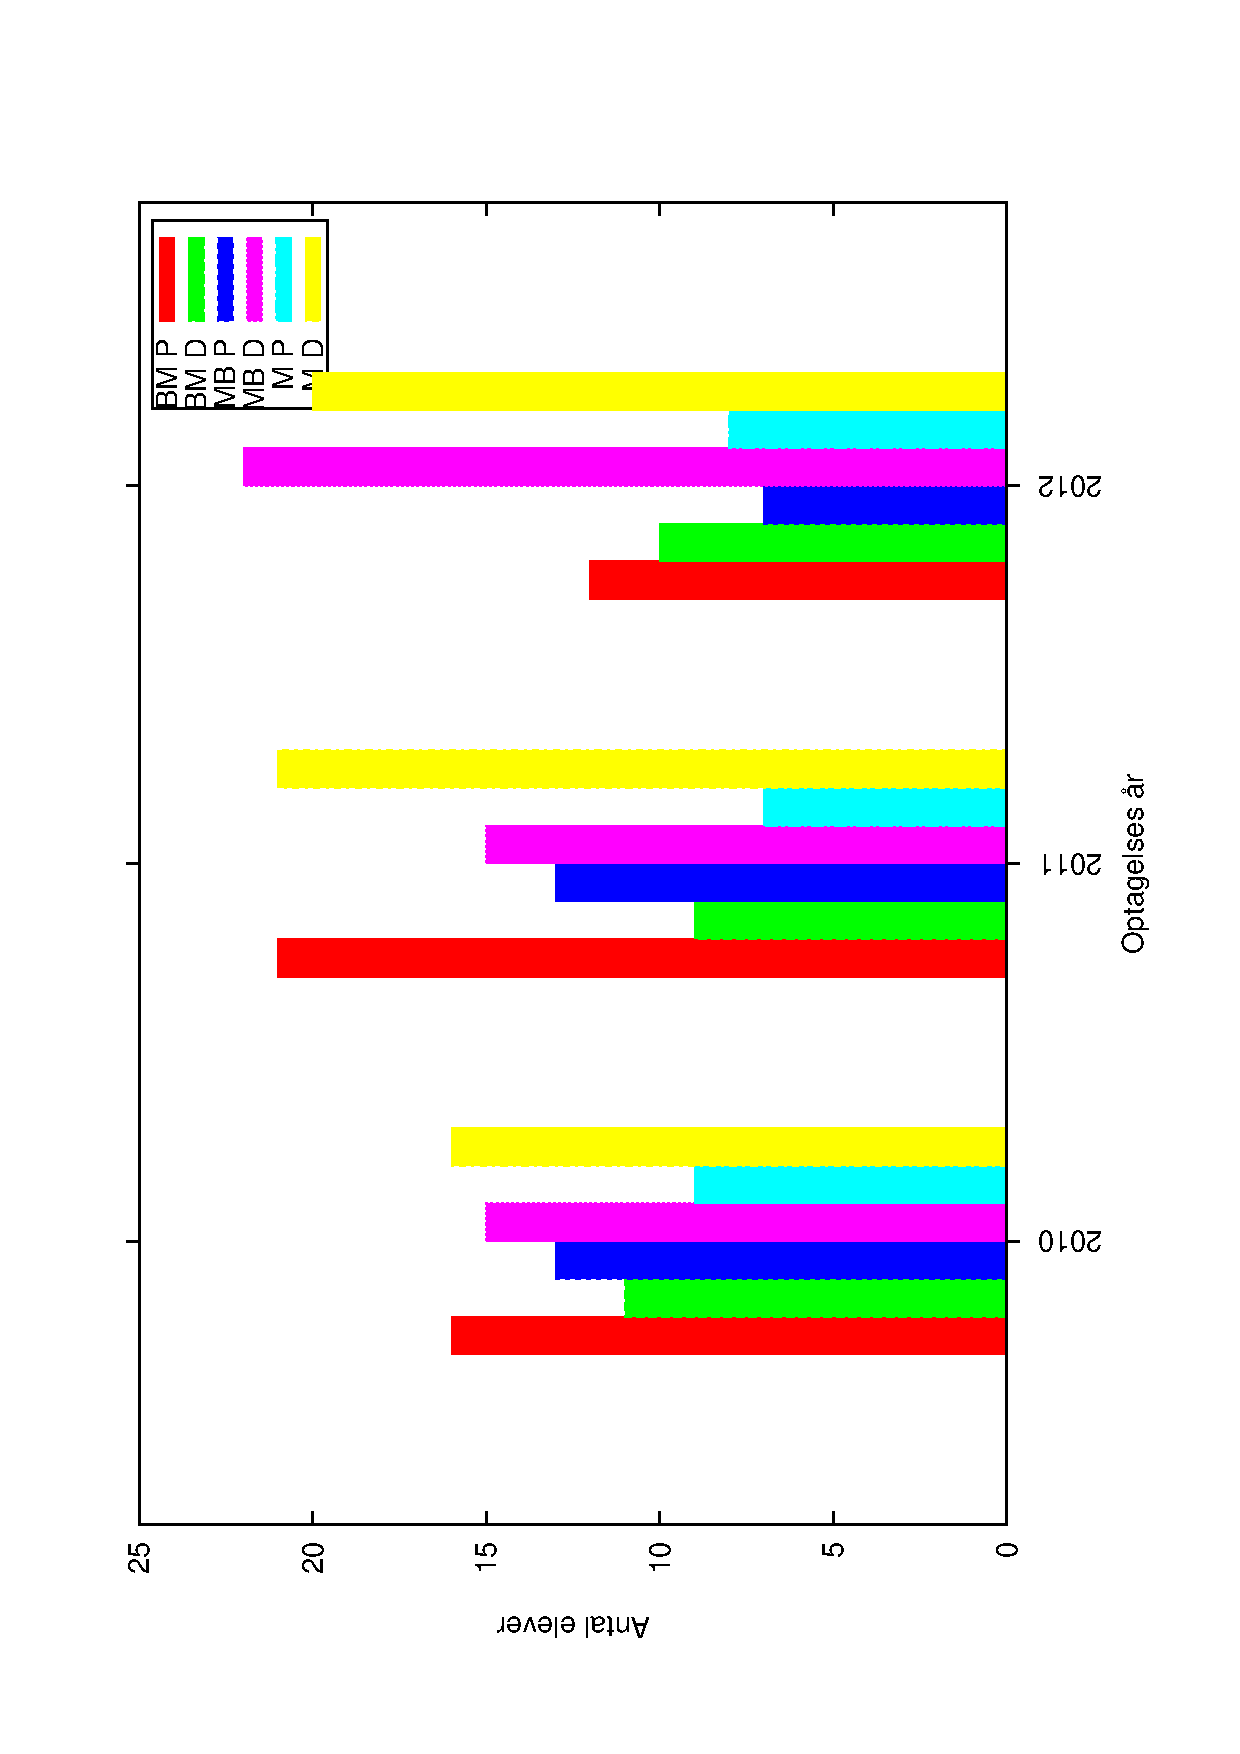
\includegraphics[width=.4\textwidth,angle=-90]{optag}
	\caption[Elevoptag p� naturvidenskabelige studieretninger]{Optag af hhv. drenge og piger p� naturvidenskabelige studieretninger inden for de sidste tre �r p� Marselisborg Gymnasium}
	\label{fig:optag}
\end{figure}

Fra \figref{optag} ser vi at antallet af optagne piger i bm-klassen svarer nogenlunde til optaget af drenge i m-klassen. Dette er dog ikke g�ldende for klasser optaget i august 2012. Her ses en klar overv�gt af drenge i b�de mb-klassen og i m-klassen. Herunder f�lger en beskrivelse af de to klasser hvori forl�bet har v�ret k�rt. Det drejer sig om nuv�rende 2.bm og nuv�rende 1.m grunden til at de to klasser er valgt er at de begge har gennemg�et forl�bet om verdensbilleder samt at de er to vidt forskellige steder i deres gymnasie forl�b og dermed er deres kognitive erkendelses niveau ogs� vidt forskelligt. 

\subsection{~bm optaget august 2011}
\label{sub:2bm}
Klassen 2.bm er en klasse der er meget domineret af det store antal piger i klassen. Klassen har en naturlig naturvidenskablig interesse som g�r i den biologiske retning hvilket ogs� afspejles i klassens valg af stuideretningsfag. Klassen har det dog generelt lidt sv�rer med de tunge naturvidenskabelige decipliner s� som fysik. Dette skyldes at de har det sv�rt med matematikken. 2.bm er pr�get meget af at der er mange elever som har det sv�rt men og at der er en del gruppe dannelse, det medvirker til at eleverne let frustreres over faglige udfordringer og at klassen let falder i f�lden med at snakke om weekenden frem for at arbejde med det stof som forel�gges dem. Fokus for denne klasse med forl�bet har v�ret at lave s�rligt elevaktiverende undervisning. For at s�tte eleverne i centrum for undervisningen og for at skabe en forundring over det verdensbillede vi har idag, og dets opst�en. 

\subsection{~m optaget august 2012}
\label{sub:1m}
Klassen 1.m er pr�get af en stor overv�gt af drenge. K�nsfordelingen i klassen er omvendt af af den fordeling der er i klassen 2.bm. Klassen 1.m er en ABB studieretning med matematik p� A niveau og fysik og kemi p� B niveau. I denne klasse har eleverne rigtig godt fat i matematikken og dermed rigitg gode foruds�tninger for at arbejde med fysik. Eleverne er meget sp�rgelystne og er naturligt meget nysgerrige, hvilket er godt for den faglige udvikling. Forl�bet blev oprindeligt gennemf�rt i 2.bm og efterf�lgende tilpasset til 1.m baseret p� de kommentarer der blev givet i hhv. den mundtlige og den skriftlige evaluering af forl�bet.

\section[JTI/MBTI]{~2 klasser ca. 60 elever og 16 personligheder}
\label{sec:2kl}
Vi har som beskrivet i \secref{NVst} har vi 2 klasser som udgangspunkt for denne opgave dermed har vi godt og vel 60 elever. Det betyder at vi har 60 forskellige personligheder som skal have stoffet serveret p� hver deres m�de. Derfor er det n�dvendigt at vide noget om hvorledes forskellige typer at personligheder skal have viden serveret for at f� det optimale ud af undervisningen. Derfor er det af vital betydning for den enkelte underviser at have kendskab til Jungs personligheds teorier \citep{jung1923psychological,JTI, Ringstad:2002}. Disse er sammen med videre udviklingen ved Myers og Briggs \citep{MBTI} blevet til at en personlighed sammens�ttes af fire pr�ferencer disse v�lges udfra nedenst�ende mods�tningspar. For en uddybende forklaring af betydningen af hver enkelt pr�ference kan \citet{Ringstad:2002} konsulteres.
\begin{center}
	\begin{tikzpicture}
		%\draw[thin, draw=LightSkyBlue, anchor=south west, step=1mm] (0,0) grid (10,10);
		%\draw[draw=blue,anchor=south west, step=5mm] (0,0) grid (10,10);
		%\draw[thick,draw=SkyBlue,anchor=south west, step=10mm] (0,0) grid (10,10);
		
		\draw[thin, black] (2,5.5) -- (8,5.5) -- (8,8) -- (2,8) -- cycle;
		\draw[thick, black] (4.7,7.7) -- (5.3,7.7);
		\draw[thick, black] (4.7,7.2) -- (5.3,7.2);
		\draw[thick, black] (4.7,6.7) -- (5.3,6.7);
		\draw[thick, black] (4.7,6.2) -- (5.3,6.2);
		
		\node[black,left] at (4.5,7.6) {Ekstrovert ({\bf E})};
		\node[black,left] at (4.5,7.2) {Sansning ({\bf S})};
		\node[black,left] at (4.5,6.7) {T�nkning ({\bf T})};
		\node[black,left] at (4.5,6.2) {Judging ({\bf J})};
		
		\node[black,right] at (5.5,7.6) {({\bf I}) Introvert};
		\node[black,right] at (5.5,7.2) {({\bf N}) INtuition};
		\node[black,right] at (5.5,6.7) {({\bf F}) F�lelse};
		\node[black,right] at (5.5,6.2) {({\bf P}) Perseption};
	\end{tikzpicture}
\end{center}

Med afs�t i denne tankegang kaldet Jungian Type Indicator (JTI) eller Myers-Briggs Type Indicator (MBTI) kan vi sammens�tte 16 forskellige personligheder. Disse fremg�r af \figref{MBTI} herunder.  P� baggrund af personlighederne i nedenst�ende skema kan vi ved hj�lp af de to midterste bogstaver i hvert personlighed definere nogle f�llestr�k dette betyder at vi f�r nogle r�de personligheder (sanse - t�nke) typer, nogle gule (sanse - f�le) typer, nogle gr�nne (intuition - f�le) typer og nogle bl� (intuition - t�nke) typer, alle beskrevet i stor detalje i \citet{Alstrup:1997,DDS:2006}.
\begin{figure}[h!]
	\centering
	\begin{tikzpicture}
		%\draw[thin, draw=LightSkyBlue, anchor=south west, step=1mm] (0,0) grid (10,10);
		%\draw[draw=blue,anchor=south west, step=5mm] (0,0) grid (10,10);
		%\draw[thick,draw=SkyBlue,anchor=south west, step=10mm] (0,0) grid (10,10);
		%
		%% DEFINE COLORS
		\definecolor{r1}{cmyk}{0.08,0.36,0.21,0}
		\definecolor{y1}{cmyk}{0.02,0.21,0.33,0}
		\definecolor{g1}{cmyk}{0.2,0.04,0.36,0}
		\definecolor{b1}{cmyk}{0.33,0.14,0.01,0}
		
		%% DEFINE COLORED REGIONS
		\draw[very thin, fill=r1] (1,1) -- (3,1) -- (3,9) -- (1,9) -- cycle;
		\draw[very thin, fill=y1] (3,1) -- (5,1) -- (5,9) -- (3,9) -- cycle;
		\draw[very thin, fill=g1] (5,1) -- (7,1) -- (7,9) -- (5,9) -- cycle;
		\draw[very thin, fill=b1] (7,1) -- (9,1) -- (9,9) -- (7,9) -- cycle;
		
		%% DRAW THE VERTICAL GRID
		\draw[very thick, black] (1,9) -- (9,9);
		\draw[very thick, black] (1,7) -- (9,7);
		\draw[very thick, black] (1,5) -- (9,5);
		\draw[very thick, black] (1,3) -- (9,3);
		\draw[very thick, black] (1,1) -- (9,1);
		
		%% DRAW THE HORIZONTAL GRID
		\draw[very thick, black] (9,1) -- (9,9);
		\draw[very thick, black] (7,1) -- (7,9);
		\draw[very thick, black] (5,1) -- (5,9);
		\draw[very thick, black] (3,1) -- (3,9);
		\draw[very thick, black] (1,1) -- (1,9);
		
		%% TOP LETTERS
		\node[black] at (2,9.5) {\fontspec[SizeFeatures={{Size=14}}]{Neo Tech Std}S};
		\node[black] at (4,9.5) {\fontspec[SizeFeatures={{Size=14}}]{Neo Tech Std}S};
		\node[black] at (6,9.5) {\fontspec[SizeFeatures={{Size=14}}]{Neo Tech Std}N};
		\node[black] at (8,9.5) {\fontspec[SizeFeatures={{Size=14}}]{Neo Tech Std}N};
		
		
		%% LEFT SIDE LETTERS
		\node[black] at (0.5,8) {\fontspec[SizeFeatures={{Size=14}}]{Neo Tech Std}I};
		\node[black] at (0.5,6) {\fontspec[SizeFeatures={{Size=14}}]{Neo Tech Std}I};
		\node[black] at (0.5,4) {\fontspec[SizeFeatures={{Size=14}}]{Neo Tech Std}E};
		\node[black] at (0.5,2) {\fontspec[SizeFeatures={{Size=14}}]{Neo Tech Std}E};
		
		%% RIGHT SIDE LETTERS
		\node[black] at (9.5,8) {\fontspec[SizeFeatures={{Size=14}}]{Neo Tech Std}J};
		\node[black] at (9.5,6) {\fontspec[SizeFeatures={{Size=14}}]{Neo Tech Std}P};
		\node[black] at (9.5,4) {\fontspec[SizeFeatures={{Size=14}}]{Neo Tech Std}P};
		\node[black] at (9.5,2) {\fontspec[SizeFeatures={{Size=14}}]{Neo Tech Std}J};
		
		%% BOTTOM LETTERS
		\node[black] at (2,.5) {\fontspec[SizeFeatures={{Size=14}}]{Neo Tech Std}T};
		\node[black] at (4,.5) {\fontspec[SizeFeatures={{Size=14}}]{Neo Tech Std}F};
		\node[black] at (6,.5) {\fontspec[SizeFeatures={{Size=14}}]{Neo Tech Std}F};
		\node[black] at (8,.5) {\fontspec[SizeFeatures={{Size=14}}]{Neo Tech Std}T};
		
		%% TYPE INDICATORS
		\node[black] at (2,8) {\fontspec[SizeFeatures={{Size=14}}]{Neo Tech Std}ISTJ};
		\node[black] at (2,6) {\fontspec[SizeFeatures={{Size=14}}]{Neo Tech Std}ISTP};
		\node[black] at (2,4) {\fontspec[SizeFeatures={{Size=14}}]{Neo Tech Std}ESTP};
		\node[black] at (2,2) {\fontspec[SizeFeatures={{Size=14}}]{Neo Tech Std}ESTJ};
		
		\node[black] at (4,8) {\fontspec[SizeFeatures={{Size=14}}]{Neo Tech Std}ISFJ};
		\node[black] at (4,6) {\fontspec[SizeFeatures={{Size=14}}]{Neo Tech Std}ISFP};
		\node[black] at (4,4) {\fontspec[SizeFeatures={{Size=14}}]{Neo Tech Std}ESFP};
		\node[black] at (4,2) {\fontspec[SizeFeatures={{Size=14}}]{Neo Tech Std}ESFJ};
		
		\node[black] at (6,8) {\fontspec[SizeFeatures={{Size=14}}]{Neo Tech Std}INFJ};
		\node[black] at (6,6) {\fontspec[SizeFeatures={{Size=14}}]{Neo Tech Std}INFP};
		\node[black] at (6,4) {\fontspec[SizeFeatures={{Size=14}}]{Neo Tech Std}ENFP};
		\node[black] at (6,2) {\fontspec[SizeFeatures={{Size=14}}]{Neo Tech Std}ENFJ};
		
		\node[black] at (8,8) {\fontspec[SizeFeatures={{Size=14}}]{Neo Tech Std}INTJ};
		\node[black] at (8,6) {\fontspec[SizeFeatures={{Size=14}}]{Neo Tech Std}INTP};
		\node[black] at (8,4) {\fontspec[SizeFeatures={{Size=14}}]{Neo Tech Std}ENTP};
		\node[black] at (8,2) {\fontspec[SizeFeatures={{Size=14}}]{Neo Tech Std}ENTJ};
	\end{tikzpicture}
	\caption[Jungs Type Indicator]{Skematisk opstilling af de 16 mulige personligheder som tillades jf. Jungs teori, \citep{jung1923psychological,JTI, Ringstad:2002, MBTI}.}
	\label{fig:MBTI}
\end{figure}
F�lles for disse fire typer at de har nogle h�ndgribelige tr�k som man som underviser b�r v�re opm�rksom p� i sin omgang med elever, og tage h�jde for n�r man planl�gger sin undervisning, og specielt elev aktiverende undervisning. De to tabeller herunder \tblref{DDS:seek} og \tblref{DDS:avoid} fremg�r det hvad det er for nogle tr�k man hos eleverne kan v�re opm�rksom p� der kan give en nogle hints til hvordan eleverne skal have opgaverne serveret og hvilke undervisningsformer man helst skal undg� for at fremme elevernes ind l�ring begge tabeller er hentet fra \citet{DDS:2006}, og farve angivelserne svare til dem angivet p� \figref{MBTI}.
\begin{table}[h!]
	\centering
	\caption[De fire ledertyper fra \citep{DDS:2006} s�ger]{De fire ledertyper fra \citet{DDS:2006}, baseret p� JTI/MBTI, s�ger:}
	\label{tbl:DDS:seek}
	\begin{tabular}{@{ } p{3.25cm} p{3.25cm} p{3.25cm} p{3.25cm} @{ }}
		\toprule[2pt]
			R�de			& Gule			& Gr�nne				& Bl�\\
			Sanse-/t�nketypen	& Sanse-/f�letypen	& Intuitions-/f�letypen	& \mbox{Intuitions-/}\mbox{t�nketypen}\\
		\midrule[1.25pt]
			At overv�ge gruppens udvikling ved hj�lp af budgetter, regnskaber, medlemstal osv.	&	At bruge afpr�vede og gennemt�nkte metoder	&	At fremme gl�de, harmoni og nyskabelse	&	At f� gruppen til at fokusere p� fremtiden\\
		\midrule[.5pt]
			At styre udgifter og handlingsplaner	&	At anvende sine erfaringer p� praktiske opgaver	&	At udf�rer arbejder der �bner mulighed for ny viden og udvikling	&	At k�de planer, metoder og modeller sammen\\
		\midrule[.5pt]
			At vise h�ndgribelige resultater	&	At fordele arbejdet retf�rdigt	&	At kommunikere p� kreative m�der	&	at finde muligheder for udvikling i gruppen\\
		\midrule[.5pt]
			At anvende afpr�vede metoder til at skabe succes	& At gennemg� planer og materialer som andre har udformet, for at finde frem til hvad der virker bedst	&	At skaffe sig indsigt i ting der er betydningsfulde for gruppens medlemmer	&	At unders�ge komplekse problemers langsigtede virkning\\
		\midrule[.5pt]	
			At l�se problemer med det samme	&		&	At arbejde p� mange forskellige m�der for at f� succes	&	At diskutere udfordrende sp�rgsm�l\\
		\bottomrule[2pt]
	\end{tabular}
\end{table}

\begin{table}[h!]
	\centering
	\caption[De fire ledertyper fra \citep{DDS:2006}]{De fire ledertyper fra \citet{DDS:2006}, baseret p� JTI/MBTI, undg�r:}
	\label{tbl:DDS:avoid}
	\begin{tabular}{@{ } p{3.25cm} p{3.25cm} p{3.25cm} p{3.25cm} @{ }}
		\toprule[2pt]
			R�de			& Gule			& Gr�nne				& Bl�\\
			Sanse-/t�nketypen	& Sanse-/f�letypen	& Intuitions-/f�letypen	& \mbox{Intuitions-/}\mbox{t�nketypen}\\
		\midrule[1.25pt]
			At deltage i alt for sociale ("langh�rede") aktiviteter	&	At anvende nye og upr�vede metoder	&	At tage sig af kontrolfunktioner s� som regnskaber	&	At g�re andres arbejde\\
		\midrule[.5pt]
			Brainstorm som ikke medf�rer noget praktisk resulatat	&	At diskuteres forskellige teorierns fordele	&	At opstille hierakier og kommandoveje	&	At kappes med andre om popularitet\\
		\midrule[.5pt]
			At opstille hypoteser om fremtiden	&	At analysere og forudsige resultater af strategiske planer	&	Intriger	&	At arbejde med administrative detaljer\\
		\midrule[.5pt]
			At anvende uafpr�vede og ikke gennemt�nkte metoder	&	At komme med kritik i et �bent forum, is�r i relation til gruppemedlemmer som de kender	&	At tage sig af papirnusseri	&	At udf�rer rutinearbejde\\
		\midrule[.5pt]
			Manglende koncentration om arbejdet	&	At behandle andre mennesker som "udskiftelige manskindele"	&		&	At deltage i alt for sociale ("langh�rede") aktiviteter\\
		\bottomrule[2pt]
	\end{tabular}
\end{table}

Basseret p� disse teorier vil vi typisk se at ca. halvdelen af de elever vi underviser vil optr�de Introverte med andre ord, de ``\emph{t�nker for at tale}'' mens de resterende er ekstroverte, de ``\emph{taler for at t�nke}''. Dette er en af grundene til at det kan v�re godt at lave sm� summe grupper da de introverte elever derved f�r l�ngere tid til at t�nke sig om. Herud vil man statistisk skulle observere at eleverne fordeler sig j�vnt mellem de fire farve kategorier, men det viser sig at i de to klasser vi har set p� er der et f�tal af bl� personligheder, hvorimod hoved v�gten er fordelt mellem r�d og gul. S�ledes klogere p� de elever som opgaven omhandler vil vi skride til problemformuleringen. 
\chapter{Problemformulering}
\label{ch:Prob}

Gennem denne teoretiske p�dagogiske opgave vil jeg tage udgangspunkt i {\bf tema B: Den faglige progression}, Og opgavens overordnedes problemformulering lyder som f�lger:\vspace{.25cm}

\section{~Problemstilling \& afgr�nsning}
\label{sec:pro}
\begin{quote}
	``{\bf Kan en underviser sikre den enkelte elevs faglige progression, i et klasserum?}''
\end{quote}\vspace{.25cm}

Problemformulering tager udgangspunkt i den problematik som blev ridset op i indledningen med at man som underviser har en ekstrem stor diversitet af forskellige elever, som har behov for at f� det faglige stof formidlet p� forskellige m�der, for at de opn�r den progression som kr�ves i gymnasieskolen. 
For at sikre at afgr�nse opgaven vil den v�re fokuseret p� tre punkter hvor man som underviser b�r have fokus p� den faglige progression.

\begin{enumerate}\itemsep=-2pt
	\item Tilrettel�ggelsen af et l�ngerevarende undervisningsforl�b.
	\item Tilrettel�ggelsen af enkelt moduler af et l�ngere varende forl�b med indbygget sekvensering.
	\item Afviklingen og evaluering af tilrettelagt undervisning i klasserummet.
\end{enumerate}

\section{~Opgavens motivation}
\label{sec:mot}
Efter mere en 20 �r i spejder bev�gelsen, er jeg nu kommet til et punkt i mit liv hvor det er p� tide at male med en st�rre pensel end blot den gammel kendte ``Learning by Doing'' som blev et mantra for John Dewey selv om det han egentlig sagde var: 
\begin{quote}
``We do not learn from experience \ldots we learn from reflecting on experience \citep{Dewey:1978}.''
\end{quote}
Det viser sig imiddelertid at  id�en om at vi l�rer noget ved at pr�ve det ikke er helt tosset, men jeg blev i �r 2012 konfronteret med fremherskende teorier fra David Kolb, som tager udgangspunkt i \citet{Dewey:1978} og udbygger denne teori til det som kommer til at hedde experiential learning eller p� dansk erfarings baseret l�ring \citep{Kolb:1984,Illeris}. Med Kolb som udgangspunkt er jeg derfor g�et til min dagige funktion som underviser ud fra de radikalkonstruktivistiske tanker som Piaget pr�senteret p� AP 2,  her er v�gten p� individet og dynamikken er en biologisk process grund id�en er at f�rst m� man modnes og herefter kan l�ringen finde sted. Dette stemmer over ens med den m�de man praktisere l�ring i f.eks. spejderbev�gelsen hvor man lader b�rn lede b�rn og hvor b�rn l�rer b�rn p� den m�de b�de udvikles b�rnene mentalt men samtidig udfordres de ogs� p� de niveau hvorp� de erkendelses m�ssigt er klar til det. Et af de vigtigste elementer vi skal tage med os fra Piaget er det ``at vi retter vores nysgerrighed mod noget (intention) og at den, der ser, spiller ind p� hvordan der ses.'' der er alts� tale om en subjektiv process. Alle disse tanker sammen med Dewey tages der alts� afs�t i gennem den leder uddannelses jeg har modtaget gennem min opv�kst i Det Danske Spejderkorps (DDS). Gennem kurser som ``\emph{Ledelse i Praksis}'' hvor disse teorier kombineres med blandt andet JTI og MBTI se \secref{2kl} og situationsbestemt  ledelse se \appref{sit:led} og process modeller som 4MAT \appref{4mat}. Alle de v�rkt�jer jeg har f�et pr�senteret gennem disse kurser har jeg kunnet anvende i mit professionelle erhvervsliv som underviser i gymnasiet. V�rkt�jerne giver mig den ledelsesm�ssige v�rkt�jskasse der g�r at jeg kan fokusere min undervisning der hvor eleverne har behov for en ekstra indsats. Dette er grunden til at jeg har valgt at pr�sentere netop dette emne og at jeg angriber det p� netop denne m�de. Kort sagt;
\begin{quote}
``Alt progression i undervisning handler om kommunikation''
\end{quote}
%Opgaven vil behandle tre konkrete emne i forhold til at sikre elevernes faglige progression.
%\begin{enumerate}\itemsep=-2pt
%	\item Med udgangspunkt i fremherskende teorier af David Kolb \citep[side 175ff, 346f] {Gympd} analyseres l�rings stilstyper og elevtyper med henblik p� at koble dette til personlighedsteori \citep{JTI, MBTI}og hvordan man ved at v�re opm�rksom p� indikatorer kan hj�lpe eleverne fremad.
%	\item Opgaven vil ligeledes med udgangspunkt i Steen Becks model og Peter Hobels diskussioner af l�rerens rolle i klasse rummet samt de didaktiske overvejelser sammeholde dette med moderne ledelsesteori, som cooperative learning og situationsbaseret ledelse \citep{Hersey1,Herse2}. Som et middel til at sikre elevernes progression
%	\item Sluttelig vil opgaven samle p� p� de to foreg�ende punkter ved at introducere planl�gningsmetoden 4MAT som et redskab der kan styrke den enkelte l�rer i didaktiseringen af enkelt moduler eller forl�b.
%\end{enumerate}
%Specielt i de naturvidenskablige fag er der behov for at t�nke anderledes i forhold til den m�de vi t�nker faglig progression p� det viser alle studier, vi kan ikke blot forholde os til den m�de Bloom opstille taksonomien p� derimod skal vi snarer kigge mode taksonomier som SOLO eller de fem E'er. Men inden vi n�r s� langt er der ting vi som undervisere er n�dt til at overveje.Kan vi f.eks. i de naturvidenskablige fag skabe denne faglige progression gennem den forberedelse s�ledes at det bliver elevernes vidensbeg�r der driver v�rket og vi dermed bev�ger os mere over mod reel unders�gelsesbaseret videnskab, (IBSE, \citet{Michelsen:2011M}). Udfordringen for den enkelte underviser er alts� i h�j grad at lave en differentiering af undervisningen s� den passer til 28 individer med yderst forskellige faglige foruds�tninger for fagene. Denne opgave kan i sit store hele l�se hvis man er opm�rksom p� sm� ting. H�r t�nkes i h�j grad p� personlighedstr�k som vil dikterer hvordan den enkelte elev bliver som elev type i forhold til D. Kolbs teori. Lige ledes skal vi som undervisere ogs� v�re ekstremt opm�rksomme p� at disse mange individer vi har i vores klasser typisk er s�dan indrettet at ca 50 \% vil favorisere h�jre hjernehalvdel frem for venstre n� de laver aktiviteter og de har typisk et h�jere abstraktions niveau end folk som anvender venstre hjernehalvdel det giver nogle udfordringer som kr�ver at man n�je udv�lger de aktiviteter man har i sinde at lave med en klasse. For at lette planl�gningen af forl�b og moduler vil jeg ogs� pr�sentere et nyt didaktiseringsv�rkt�j kaldet 4MAT modellen, som virker i praksis - og som hj�lper med at f� valgt hensigtsm�ssige aktiviteter i forhold til klassens elever. Selve opgaven tager sit udgangspunkt i et forl�b om verdensbilleder. Forl�bet er gennemf�rt i to klasser uafh�ngigt af hinanden og l�ringsudbyttet har i begge klasser v�ret h�jt.

%Problemformuleringen og de tre cases der her tages op bygger p� en interesse for ledelse og ledelsesteori som v�rkt�j til at hj�lpe elever videre fagligt s�vel som mentalt. Det er mit indtryk at de fleste �ldre l�rer i gymnasieskolen t�nker mindre p� de didaktiske p�dagogiske teorier efterh�nden som de bliver mere og mere tr�nede i at undervise. Dette kan v�re et udtryk for at man er ligeglad med teorien eller at den bliver routine. Jeg er af den holdning at hvis man kan give underviserne nogle v�rkt�jer som virker s� er de ogs� mere villige til at have teorien med i deres daglige arbejde.

%Herunder vil opgaven besk�ftige sig med elevtyper baseret p� David Kolbs teorier (DKT) \citep[side 175ff] {Gympd}. Endvidere vil opgaven inddrage personlighedstype indikatorer baseret p� Jungs teorier (Jungs Type Indicator = JTI) \citep{JTI} samt Myers-Briggs Type indicator (MBTI) \citep{MBTI}. Opgaven vil ogs� inddrage moderne gruppeledelses teorier s� som Cooperative Learning (CL) og situationsbestemt ledelse (SL) \citep{Hersey1,Herse2} sluttelig vil opgaven kigge p� en praktisk oms�ttelse af Kolbs teorier denne kaldes 4MAT modellen.
\chapter[Progression og Metode i opgaven]{PROGRESSION OG METODE}
\label{ch:ProgMet}
Udgangspunktet for denne opgave er et forl�b med titlen ``Verdensbilleder'' (se forl�bsplan \appref{Verden}). Forl�bet er gennemf�rt to gange i forskellige klasser begge 2. �rige B-niveau hold hvor den ene var en 2.g klasse p� tidspunktet for gennemf�rselen mens den anden var en 1.g klasse. Da forl�bene blev gennemf�rt uafh�ngigt af hinanden er der inddraget erfarringer fra det f�rste forl�b i tilrettel�ggelsen af det andet forl�b og modulplanen som er fremlagt i \appref{Verden}. Indledningsvist vil der forekomme en begrebsafklaring samt et afsnit om elevtyper og l�ringsstile for klassen 1.m. P� baggrund af dette vil de didaktiske-teoretiske overvejelser bag forl�bet samt egne overvejelser om elevernes faglige progression blive behandlet.
Opgavens emperi bygger p� observationer og vurderinger som er foretaget i forbindelse med gennemf�rsel af forl�bet.  Indsamlingen og behandlingen af emperi er inspireret af og struktureret i henhold til Bj�rndals Vurderings kube \citep{Bjrndal:2003}. Bj�rndals Vurderingskube best�r af en intentionsdel og en realiseringsdel (se \figref{Kube}). 
\begin{figure}[htb]
	\centering
	\begin{tikzpicture}
		%\draw[very thin, lightgray, step=1mm] (0,0) grid (10,10);
		%\draw[thin, gray, step=5mm] (0,0) grid (10,10);
		%\draw[thick, darkgray, step=10mm] (0,0) grid (10,10);
		
		% DRAW THE CUBE
		\filldraw[fill=blue!10!white, draw=blue!10!black] (1,1) -- (9,1) -- (9,6) -- (1,6) -- cycle;
		\filldraw[fill=blue!10!white, draw=blue!10!black] (9,6) -- (8,8) -- (2,8) -- (1,6) -- cycle; 
		\draw[blue!10!black] (5,1) -- (5,8) (1,3) -- (9,3) (1,4) -- ( 9,4);
		\draw[very thick, black, <->] (1,.75) -- (9,.75);
		\draw[very thick, black, <->] (.75,1) -- (.75,6);
		\node at (5,.5) {Empirisk vurdering};
		\node[rotate=90] at (.5,3.5) {Teoretisk vurdering}; 
		\node[left] at (4,7) {1. Intentioner};
		\node[left] at (7.5,7) {2. Realisering};
		\node[left] at (4.5,5.5) {a) Foruds�tninger for }; 
		\node[left] at (4.7,5) {p�dagogisk praksis};
		\node[left] at (4.7,3.5) {b) P�dagogisk process};
		\node[left] at (4.7,2.5) {c) Resultat af p�dago- }; 
		\node[left] at (3.6,2) {gisk praksis};
		
		\node[left] at (8.5,5.5) {a) Foruds�tninger for }; 
		\node[left] at (8.7,5) {p�dagogisk praksis};
		\node[left] at (8.7,3.5) {b) P�dagogisk process};
		\node[left] at (8.7,2.5) {c) Resultat af p�dago- }; 
		\node[left] at (7.6,2) {gisk praksis};
	\end{tikzpicture}
	\caption[Bj�rndals vurderingskube]{Vuderingskuben af \citet{Bjrndal:2003}}
	\label{fig:Kube}
\end{figure}

 Intentionsdelen forholder sig til de tanker og planer man inddrog i forbindelse med planl�gningen mens realisationen forholder sig til hvad der rentfaktisk skete i  praksis \citep{Bjrndal:2003}. Afslutningsvis vil der v�re en konklusion som s�ger at perspektivere opgaven til den fremtidige uddannelsesm�ssige ramme.
 
\chapter{Begrebsafklaring}
\label{ch:Beg}
\section{~L�ring}
\label{sec:teach}
Denne opgaves opfattelse af l�ring er baseret p� David Kolbs - Erfaringsbasserede l�ring \citep{Kolb:1984}. Kolbs teorier tager sit udgangspunkt i bl.a. John Deweys ``Learning by doing'' \citep{Dewey:1978} -- hvor fokus l�gges p� handlen og ageren i verden. Grundlaget for at v�lge denne l�ringsopfattelse er at den erkendelsesbasserede rationelle l�ring oftest ligger i god tr�d med den naturvidenskablige m�de at t�nke p�. Endvidere er det et udtryk for den baggrund jeg har fra spejderbev�gelsen hvor Deweys mantra ``Learning by doing'' altid har v�ret et motto. Foruden Dewey bygger kolbs teori p� andre l�ringsteoretikkere som Kurt Lewin og Jean Piaget, som alle ser l�ring som en natur sp�ndings- og konfliktfyldt aktivitet. De har hveris�r deres konflikt par. Hvor Dewey  og Lewin arbejder med mods�tningen mellem indtryk og tanker eller id�er alts� den konkrete erfaring mod de abstrakte begreber. S� arbejder Piaget med l�ringen som vekselvirkningen mellem akkommodation af id�er og assimilation af erfaring alts� en vekselvirkning mellem den aktive eksperimenteren og de reflekterende observationer. Dette giver anledning til den vandrette og den horisontale akse i Kolbs l�ringsmodel (se \figref{kolb1}) 
\begin{figure}[hbt]
	\centering
	\begin{tikzpicture}
		%\draw[very thin, lightgray, step=1mm] (0,0) grid (10,10);
		%\draw[thin, gray, step=5mm] (0,0) grid (10,10);
		%\draw[thick, darkgray, step=10mm] (0,0) grid (10,10);
		
		% WRITE THE FOUR POINTS
		\node at (0,5.3) {Aktiv};
		\node at (0,5) {eksperimenteren};
		
		\node at (5,10) {konkret};
		\node at (5,9.7) {erfaring};
		
		\node at (10,5.3) {Reflekterende};
		\node at (10,5) {observation};
		
		\node at (5,.3) {Abstrakt};
		\node at (5,0) {begrebsdannelse};
		
		% PLACE ROUND ARROWS
		\draw[very thick, blue!40!white, ->, rotate=-90] (-.5,4) arc (0:-90:4cm);
		\draw[very thick, blue!40!white, ->, rotate=180] (0,-5.75) arc (0:-90:4cm);
		\draw[very thick, blue!40!white, ->, rotate=90] (9.75,-6) arc (0:-90:4cm);
		\draw[very thick, blue!40!white, ->, rotate=0] (10,4.5) arc (0:-90:4cm);

		% DRAW VERTICAL AND HORIZONTAL ARROW
		\draw[very thick, blue!80!black, <->] (5,.5) -- (5,9.5);
		\draw[very thick, blue!80!black, <->] (1.5,5) -- (9,5);
		
		% DRAW NOTES
		\node[draw=white, fill=white, text=black] at (5,2) {Begribelse via};
		\node[draw=white, fill=white, text=black] at (5,1.5) {BEGREBSBASERET REFLEKSION};
		
		\node[draw=white, fill=white, text=black] at (5,8.5) {Begribelse via};
		\node[draw=white, fill=white, text=black] at (5,8.0) {UMIDDELBAR OPLEVELSE};
		
		\node[draw=white, fill=white, text=black] at (3,5.3) {Omdannelse via};
		\node[draw=white, fill=white, text=black] at (3,4.7) {AKTIV HANDLEN};
		
		\node[draw=white, fill=white, text=black] at (7,5.3) {Omdannelse via};
		\node[draw=white, fill=white, text=black] at (7,4.7) {MENINGSTILSKRIVELSE};
		
		\node[red] at (3,7) {Akkumolativ erkendelse};
		\node[red] at (7,7) {Divergent erkendelse};
		\node[red] at (3,3) {Konvergent erkendelse};
		\node[red] at (7,3) {Assimilativ erkendelse};
	\end{tikzpicture}
	\caption[Kolbs l�ringsmodel]{Kolbs l�ringsmodel \citep[side 42]{Kolb:1984} og \citep[side 177]{Gympd}}
	\label{fig:kolb1}
\end{figure}
Det nye i Kolbs l�ringsmodel i forhold til tidligere er at Kolb introducere en individuel erfarings tilgang til det kognitive begrebs apparat som Piaget og mentalismen st�r for. og derved bringer sociokulturalismen ind i l�ringen gennem praksisf�llesskaber. 

Tager vi udgangspunkt i \figref{kolb1} kan denne illustrere hvorledes en elev er n�dt til at bearbejde et f�nomen f�r der er tale om 


%Opgavens tilgang til l�ring baseres i h�j grad p� det rationalisme, med baggrund i Kolbs l�rings teorier. Et af de tidligste mantraer inden for denne l�rings teori er ``\emph{Learning by doing}'' som stammer fra John Dewey 
\begin{table}
	\centering
	\caption[Kolbs l�ringstilgange]{Kolbs L�ringstilgange \citep[side 347]{Gympd}}
	\begin{tabular}{l l p{7cm}}
		\toprule[2pt]
		Erkendelsesform & L�ringstilgang & Egenskaber hos den l�rende\\
		\midrule
		\multirow{4}{*}{Divergent erkendelse} 	& \multirow{2}{*}{Konkret erfaring} 			& Udviklet forestillingsevne\\ 
										&									& God til at udvikle id\'eer og unders�ge ud fra forskellige perspektiver\\
										& \multirow{2}{*}{Reflekterende observation}	& Interesserer sig for mennesker\\
										&									&  Bredt interessefelt (kulturelt) \\
		\midrule
		\multirow{3}{*}{Assimilativ erkendelse}	& Abstrakt begrebsligg�relse				& Udviklet evne til at danne teoretiske modeller\\
										& \multirow{2}{*}{Reflekterende observation}	& God til induktiiv r�sonnering\\
										&									& Interesse for abstract begreber frem for mennesker\\
		\midrule
		\multirow{4}{*}{Konvergent erkendelse}	& \multirow{2}{*}{Abstrakt begrebsligg�relse}	& St�rk i praktisk anvendelse af id\'eer\\
										&									& God til deduktivt r�sinnement\\
										& \multirow{2}{*}{Aktiv eksperimenteren}		& Ikke f�lelsesbetonet\\
										&									& Sn�vert interessefelt\\
		\midrule
		\multirow{4}{*}{Akkumulativ erkendelse}	& \multirow{2}{*}{Konkret erfaring}			& Allerbedst til at handle\\
										&									& L�ber gerne en risiko/er chancerytter\\
										& \multirow{2}{*}{Aktiv esperimenteren}		& God til at handle ``i nuet''\\
										&									& L�ser problemer intuitivt\\
		\bottomrule[2pt]
	\end{tabular}
\end{table}


\section{~Motivation}
\label{sec:mot}









\chapter{L�ringsstile i klassen}
\label{ch:LT}
\section{Elevtyper}
\label{sec:ET}
\chapter{Jungs Type Indikator}
\label{ch:JTI}
I begyndelsen af 1920'erne udgav den Carl Gustav Jung en bog som omhandlede typologiske teorier, denne blev i 1923 oversat til engelsk hvor den fik titlen "Psykological Types". I denne bog fremstillede Jung fire overordnede psykologiske egenskaber som vi opfatter verden igennem: sansning, intuition, f�ling og t�nkning. Men kun en af disse er dominant det meste af tiden \citep{Ringstad:2002}. Disse teorier af Jung danner grundlaget for det vi idag kender som Jungs type indikator (JTI). Efter at Jung havde udgivet sit v�rk blev det forarbejdet af Katharine Cook Briggs og Isabel Briggs Myers og i 1962 udgav de deres type indikator under navnet Myers Briggs Type Indikator (MBTI). B�de JTI og MBTI bygger p� et system hvor man afd�kker personlighedens pr�ferencer for forskellige ting man stille fire kategorier op hvor der er to valg muligheder i hver.

\begin{center}
	\begin{tikzpicture}
		%\draw[thin, draw=LightSkyBlue, anchor=south west, step=1mm] (0,0) grid (10,10);
		%\draw[draw=blue,anchor=south west, step=5mm] (0,0) grid (10,10);
		%\draw[thick,draw=SkyBlue,anchor=south west, step=10mm] (0,0) grid (10,10);
		
		\draw[thin, black] (2,5.5) -- (8,5.5) -- (8,8) -- (2,8) -- cycle;
		\draw[thick, black] (4.7,7.7) -- (5.3,7.7);
		\draw[thick, black] (4.7,7.2) -- (5.3,7.2);
		\draw[thick, black] (4.7,6.7) -- (5.3,6.7);
		\draw[thick, black] (4.7,6.2) -- (5.3,6.2);
		
		\node[black,left] at (4.5,7.6) {Ekstrovert ({\bf E})};
		\node[black,left] at (4.5,7.2) {Sansning ({\bf S})};
		\node[black,left] at (4.5,6.7) {T�nkning ({\bf T})};
		\node[black,left] at (4.5,6.2) {Judging ({\bf J})};
		
		\node[black,right] at (5.5,7.6) {({\bf I}) Introvert};
		\node[black,right] at (5.5,7.2) {({\bf N}) INtuition};
		\node[black,right] at (5.5,6.7) {({\bf F}) F�lelse};
		\node[black,right] at (5.5,6.2) {({\bf P}) Perseption};
	\end{tikzpicture}
\end{center}
Dette giver 16 mulige kombinationer som er vist p� \figref{MBTI} herunder. 
\begin{figure}[h!]
	\centering
	\begin{tikzpicture}
		%\draw[thin, draw=LightSkyBlue, anchor=south west, step=1mm] (0,0) grid (10,10);
		%\draw[draw=blue,anchor=south west, step=5mm] (0,0) grid (10,10);
		%\draw[thick,draw=SkyBlue,anchor=south west, step=10mm] (0,0) grid (10,10);
		%
		%% DEFINE COLORS
		\definecolor{r1}{cmyk}{0.08,0.36,0.21,0}
		\definecolor{y1}{cmyk}{0.02,0.21,0.33,0}
		\definecolor{g1}{cmyk}{0.2,0.04,0.36,0}
		\definecolor{b1}{cmyk}{0.33,0.14,0.01,0}
		
		%% DEFINE COLORED REGIONS
		\draw[very thin, fill=r1] (1,1) -- (3,1) -- (3,9) -- (1,9) -- cycle;
		\draw[very thin, fill=y1] (3,1) -- (5,1) -- (5,9) -- (3,9) -- cycle;
		\draw[very thin, fill=g1] (5,1) -- (7,1) -- (7,9) -- (5,9) -- cycle;
		\draw[very thin, fill=b1] (7,1) -- (9,1) -- (9,9) -- (7,9) -- cycle;
		
		%% DRAW THE VERTICAL GRID
		\draw[very thick, black] (1,9) -- (9,9);
		\draw[very thick, black] (1,7) -- (9,7);
		\draw[very thick, black] (1,5) -- (9,5);
		\draw[very thick, black] (1,3) -- (9,3);
		\draw[very thick, black] (1,1) -- (9,1);
		
		%% DRAW THE HORIZONTAL GRID
		\draw[very thick, black] (9,1) -- (9,9);
		\draw[very thick, black] (7,1) -- (7,9);
		\draw[very thick, black] (5,1) -- (5,9);
		\draw[very thick, black] (3,1) -- (3,9);
		\draw[very thick, black] (1,1) -- (1,9);
		
		%% TOP LETTERS
		\node[black] at (2,9.5) {\fontspec[SizeFeatures={{Size=14}}]{Neo Tech Std}S};
		\node[black] at (4,9.5) {\fontspec[SizeFeatures={{Size=14}}]{Neo Tech Std}S};
		\node[black] at (6,9.5) {\fontspec[SizeFeatures={{Size=14}}]{Neo Tech Std}N};
		\node[black] at (8,9.5) {\fontspec[SizeFeatures={{Size=14}}]{Neo Tech Std}N};
		
		
		%% LEFT SIDE LETTERS
		\node[black] at (0.5,8) {\fontspec[SizeFeatures={{Size=14}}]{Neo Tech Std}I};
		\node[black] at (0.5,6) {\fontspec[SizeFeatures={{Size=14}}]{Neo Tech Std}I};
		\node[black] at (0.5,4) {\fontspec[SizeFeatures={{Size=14}}]{Neo Tech Std}E};
		\node[black] at (0.5,2) {\fontspec[SizeFeatures={{Size=14}}]{Neo Tech Std}E};
		
		%% RIGHT SIDE LETTERS
		\node[black] at (9.5,8) {\fontspec[SizeFeatures={{Size=14}}]{Neo Tech Std}J};
		\node[black] at (9.5,6) {\fontspec[SizeFeatures={{Size=14}}]{Neo Tech Std}P};
		\node[black] at (9.5,4) {\fontspec[SizeFeatures={{Size=14}}]{Neo Tech Std}P};
		\node[black] at (9.5,2) {\fontspec[SizeFeatures={{Size=14}}]{Neo Tech Std}J};
		
		%% BOTTOM LETTERS
		\node[black] at (2,.5) {\fontspec[SizeFeatures={{Size=14}}]{Neo Tech Std}T};
		\node[black] at (4,.5) {\fontspec[SizeFeatures={{Size=14}}]{Neo Tech Std}F};
		\node[black] at (6,.5) {\fontspec[SizeFeatures={{Size=14}}]{Neo Tech Std}F};
		\node[black] at (8,.5) {\fontspec[SizeFeatures={{Size=14}}]{Neo Tech Std}T};
		
		%% TYPE INDICATORS
		\node[black] at (2,8) {\fontspec[SizeFeatures={{Size=14}}]{Neo Tech Std}ISTJ};
		\node[black] at (2,6) {\fontspec[SizeFeatures={{Size=14}}]{Neo Tech Std}ISTP};
		\node[black] at (2,4) {\fontspec[SizeFeatures={{Size=14}}]{Neo Tech Std}ESTP};
		\node[black] at (2,2) {\fontspec[SizeFeatures={{Size=14}}]{Neo Tech Std}ESTJ};
		
		\node[black] at (4,8) {\fontspec[SizeFeatures={{Size=14}}]{Neo Tech Std}ISFJ};
		\node[black] at (4,6) {\fontspec[SizeFeatures={{Size=14}}]{Neo Tech Std}ISFP};
		\node[black] at (4,4) {\fontspec[SizeFeatures={{Size=14}}]{Neo Tech Std}ESFP};
		\node[black] at (4,2) {\fontspec[SizeFeatures={{Size=14}}]{Neo Tech Std}ESFJ};
		
		\node[black] at (6,8) {\fontspec[SizeFeatures={{Size=14}}]{Neo Tech Std}INFJ};
		\node[black] at (6,6) {\fontspec[SizeFeatures={{Size=14}}]{Neo Tech Std}INFP};
		\node[black] at (6,4) {\fontspec[SizeFeatures={{Size=14}}]{Neo Tech Std}ENFP};
		\node[black] at (6,2) {\fontspec[SizeFeatures={{Size=14}}]{Neo Tech Std}ENFJ};
		
		\node[black] at (8,8) {\fontspec[SizeFeatures={{Size=14}}]{Neo Tech Std}INTJ};
		\node[black] at (8,6) {\fontspec[SizeFeatures={{Size=14}}]{Neo Tech Std}INTP};
		\node[black] at (8,4) {\fontspec[SizeFeatures={{Size=14}}]{Neo Tech Std}ENTP};
		\node[black] at (8,2) {\fontspec[SizeFeatures={{Size=14}}]{Neo Tech Std}ENTJ};
	\end{tikzpicture}
	\caption[Jungs Type Indicator]{Skematisk opstilling af de 16 mulige personligheder som tillades jf. Jungs teori, \citep{Ringstad:2002}.}
	\label{fig:MBTI}
\end{figure}

Skeler man til disse personlighedstyper n�r man sammens�tter grupper vil man opn� mere harmoniske grupper hvori eleverne vil kunne opn� bedre resultater fordi man som underviser kan give gruppe en bedre dynamik hvor eleverne ikke som udgangspunkt vil modarbejde hinanden men naturligt vil kunne indg� et konstruktivt samarbejde. Fra \figref{MBTI} ses det at type matricen har et lag mere, den er farvekodet og dette er ikke tilf�ldige farver. Disse farver kommer fra \citet[s. 121]{DDS:2006}, her arbejdes der med de fire ledertyper. Ledertyperne er kategoriseret p� baggrund af de to midderste bogstaver i JTI/MBTI typen. S�ledes kan der opbygges f�lgende fire kategorier, i \tblref{DDS:seek} s�ger alle typerne:

\begin{table}[h!]
	\centering
	\caption[De fire ledertyper fra \citep{DDS:2006} s�ger]{De fire ledertyper fra \citet{DDS:2006}, baseret p� JTI/MBTI, s�ger:}
	\label{tbl:DDS:seek}
	\begin{tabular}{@{ } p{3.25cm} p{3.25cm} p{3.25cm} p{3.25cm} @{ }}
		\toprule[2pt]
			R�de			& Gule			& Gr�nne				& Bl�\\
			Sanse-/t�nketypen	& Sanse-/f�letypen	& Intuitions-/f�letypen	& \mbox{Intuitions-/}\mbox{t�nketypen}\\
		\midrule[1.25pt]
			At overv�ge gruppens udvikling ved hj�lp af budgetter, regnskaber, medlemstal osv.	&	At bruge afpr�vede og gennemt�nkte metoder	&	At fremme gl�de, harmoni og nyskabelse	&	At f� gruppen til at fokusere p� fremtiden\\
		\midrule[.5pt]
			At styre udgifter og handlingsplaner	&	At anvende sine erfaringer p� praktiske opgaver	&	At udf�rer arbejder der �bner mulighed for ny viden og udvikling	&	At k�de planer, metoder og modeller sammen\\
		\midrule[.5pt]
			At vise h�ndgribelige resultater	&	At fordele arbejdet retf�rdigt	&	At kommunikere p� kreative m�der	&	at finde muligheder for udvikling i gruppen\\
		\midrule[.5pt]
			At anvende afpr�vede metoder til at skabe succes	& At gennemg� planer og materialer som andre har udformet, for at finde frem til hvad der virker bedst	&	At skaffe sig indsigt i ting der er betydningsfulde for gruppens medlemmer	&	At unders�ge komplekse problemers langsigtede virkning\\
		\midrule[.5pt]	
			At l�se problemer med det samme	&		&	At arbejde p� mange forskellige m�der for at f� succes	&	At diskutere udfordrende sp�rgsm�l\\
		\bottomrule[2pt]
	\end{tabular}
\end{table}

P� samme vis har de fire ledertyper ogs� ting som de undg�r, disse ting fremg�r af \tblref{DDS:avoid}

\begin{table}[h!]
	\centering
	\caption[De fire ledertyper fra \citep{DDS:2006}]{De fire ledertyper fra \citet{DDS:2006}, baseret p� JTI/MBTI, undg�r:}
	\label{tbl:DDS:avoid}
	\begin{tabular}{@{ } p{3.25cm} p{3.25cm} p{3.25cm} p{3.25cm} @{ }}
		\toprule[2pt]
			R�de			& Gule			& Gr�nne				& Bl�\\
			Sanse-/t�nketypen	& Sanse-/f�letypen	& Intuitions-/f�letypen	& \mbox{Intuitions-/}\mbox{t�nketypen}\\
		\midrule[1.25pt]
			At deltage i alt for sociale ("langh�rede") aktiviteter	&	At anvende nye og upr�vede metoder	&	At tage sig af kontrolfunktioner s� som regnskaber	&	At g�re andres arbejde\\
		\midrule[.5pt]
			Brainstorm som ikke medf�rer noget praktisk resulatat	&	At diskuteres forskellige teorierns fordele	&	At opstille hierakier og kommandoveje	&	At kappes med andre om popularitet\\
		\midrule[.5pt]
			At opstille hypoteser om fremtiden	&	At analysere og forudsige resultater af strategiske planer	&	Intriger	&	At arbejde med administrative detaljer\\
		\midrule[.5pt]
			At anvende uafpr�vede og ikke gennemt�nkte metoder	&	At komme med kritik i et �bent forum, is�r i relation til gruppemedlemmer som de kender	&	At tage sig af papirnusseri	&	At udf�rer rutinearbejde\\
		\midrule[.5pt]
			Manglende koncentration om arbejdet	&	At behandle andre mennesker som "udskiftelige manskindele"	&		&	At deltage i alt for sociale ("langh�rede") aktiviteter\\
		\bottomrule[2pt]
	\end{tabular}
\end{table}
Farvelaget i \figref{MBTI} giver os alts� informationer om hvilke arbejdsopgaver vi b�r give den enkelte elev i et gruppearbejde. Dette benyttes allerede n�r man f.eks. sammens�tter grupper efter Cooperative Learning (CL) princippet. Her p�l�gger man de dygtigste elever at hj�lpe de mindre dygtige elever, her ved bliver de dygtige elever bedre da de formidler stoffet for deres kammerater, og de mindre dygtige elever bliver ogs� bedre da de f�r  mere undervisning. Hermed sikres god progression som f�lge af en differentiering af undervisningen. Hvis man udvider den CL tanke til gruppe arbejde samtidig med at man bevidst anvender JTI/MBTI i forhold til gruppe dannelse opn�r man at eleverne i gruppe arbejdet opn�r en slags team-sprit. Herved opn�es en endnu h�jere grad af faglig progression da eleverne opn�r en sags symbiose grundet i den m�de hvorp� de vil kommunikere med hinanden.
\chapter[Didaktisk-teoretiske overvejelser om forl�bet]{Didaktisk-teoretiske overvejelser}
\label{ch:DTOF}
I det f�lgende kapitel vil vi se n�rmere p� det didaktiske udgangspunkt for det valgte undervisningsforl�b. Forl�bet tager sit udgangs punkt i emnet verdensbilleder, faget l�replan skriver f�lgende:
\begin{quote}
``{\bf Fysikkens bidrag til det naturvidenskablige verdensbillede}:\\
	\begin{itemize}
		\item Grundtr�k af den nuv�rende fysiske beskrivelse af universet og dets udviklingshistorie med fokus p� Det kosmologiske princip og universets udvidelse, herunder spektrallinjers r�dforskydning
		\item Jorden som planet i solsystemet som grundlag for forklaring af umiddelbart observerbare naturf�nomener
	\end{itemize}
	\begin{flushright}\citet[\href{https://www.retsinformation.dk/Forms/R0710.aspx?id=132647\#B24}{uvm.dk}]{FysB}''\end{flushright}
\end{quote}

Dette er et emne som oftest negligeres af fysik undervisere da disse ikke mener at det er synderligt interessant. Derimod har jeg taget udgangspunkt i at hvis man ikke forst�r hvorfra vores verdens syn er kommet s� forst�r man heller ikke hvor vi bev�ger os hen. Citatet fra l�replanen herover danner rammen om den faglige tilgang til forl�bet, mens den didaktiske ramme var pr�get af fokuspunktet elevaktiverende undervisning. I de f�lgende \secref{FTU} om forl�bets teoretiske udgangspunkt og \secref{DFP} om den faglige progression gennemg�es den teoretiske baggrund for forl�bet. Forl�bets ramme var kapitel 3 i FysikABbogen 1 af \citet{Benoni:2011}. Samt ovenst�ende uddrag af l�replanen for Fysik B. 

\section{Forl�bets teoretiske udgangspunkt}
\label{sec:FTU}
Gennem dette forl�b var �nsket at arbejde med elev aktiverende undersvisning.  Udgangspunktet hvor eleven er i fokus l�gger automatisk op til at vi vil bev�ge os i retning af tanker som findes hos Dewey under mantraet ``Learning by doing'', men det er ikke blot gennem selv at arbejde med arbejdet at eleven opn�r en st�rre kognitiv forst�else af stoffet dette g�res ved at sende eleven p� en erfaringsbaseret rejse gennemstoffet. Hvorved vi g�r fra Deweys om end lidt firkantede tilgang til l�ring over og dykker ned i en mere forfinet teori som den udviklet af David Kolb. Kolbs l�ringsteorier er en udvidelse af Deweys teorier og kan beskrives som erfarringsbaseret l�ring, \citep{Illeris}. I artiklen af \citet{Illeris} fremg�r det at vi skal passe p� med blot at anvende Kolbs l�ringsstile. Det fremg�r endvidere at Kolb testede sine teorier p� en r�kke af studerende i USA, her s� man et m�nster hvorefter de studerende fordeltes. Det viste sig at studerende p� fagene psykologi, polotogi og historie endte med ligge mellem den konkrete oplevelse og den reflekterende observation i \figref{kolb1}. Studerende p� fag som �konomi og sociologi havnede mellem den reflekterende observation og den abstrakte begrebsligg�relse, se igen \figref{kolb1}, studerende fra de naturvidenskablige fag fysik, kemi og matematik endte i kategorien abstrakt begrebsligg�relse. Ingeni�rer og Sygeplejersker ligger typisk mellem den abstrakt begrebsligg�relse og den aktive eksperimenteren p� \figref{kolb1} og sidst men ikke mindst havde vi studerende i handelssektoren som endte mellem den aktive eksperimenteren og den konkrete oplevelse. Derfor udviklede Kolb nogle erkendelses-niveauer i sin teori disse koblede de fire hovede omr�der, derved fik psykologi, polotogi og historie koblet den divergente erkendelse p�. �konomi og sociologi blev tilskrevet en assimilativ erkendelse. Ingeni�rer og sygeplejersker fik tilskrevet konvergent erkendelse og de naturvidenskabelige studerende l� imellem den assimilative erkendelse og den konvergente erkendelse dette blev til begribelse via forst�else. Sluttelig blev handelssektoren koblet med den akkomodative erkendelse, \citet{Illeris}.
\begin{figure}[h!]
	\centering
	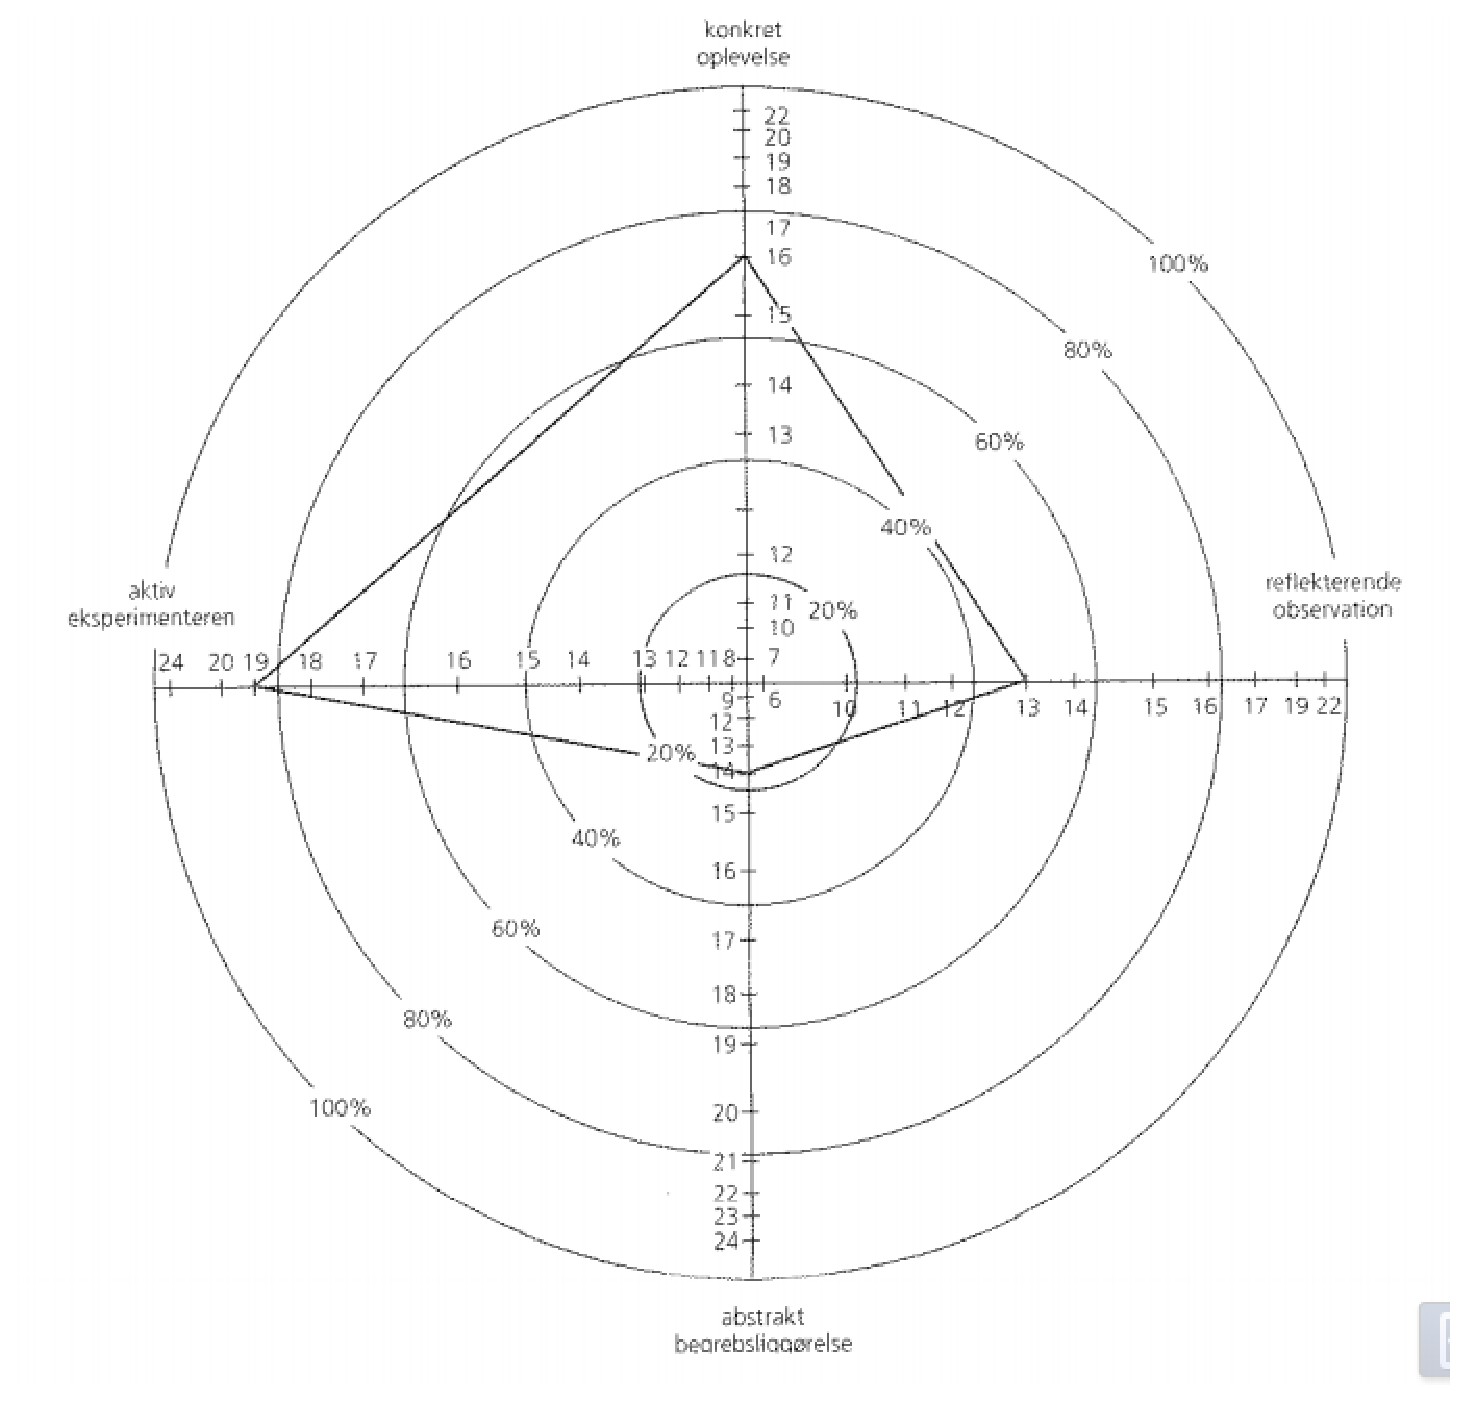
\includegraphics[width=.5\textwidth]{kolbstyle}
	\caption[M�ling af L�ringsstil]{Her vises resultatet af en l�ringsstils analyse af en socialarbejder, \citep{Illeris}}
	\label{fig:kolb2}
\end{figure}
Det skal dog hertil siges at det ikke er en ligefrem sag at bestemme en persons l�ringsstil. Af \figref{kolb2} fremg�r det at en l�ringsstil n�r den er bestemt kan illustreres som en polygon i en slags ``pol�rtkoordinatsystem''. Der findes flere tests som kan fastsl� en persons foretrukne l�ringsstil, jeg har f�et min egen testet gennem 4MAT. Det er meget vigtigt for elevernes indl�ring af stoffet at man har stort kendskab til sin egen l�ringsstil og endvidere til andre typer af l�ringsstile, da dette er vigtigt for opn�elsen af god l�ring for eleverne. 


\section{Den faglige progression}
\label{sec:DFP}
\chapter[Analyse og diskussion af den faglige progression]{Analyse og diskussion}
\label{ch:AogD}
\chapter{Evaluering og refleksioner}
\label{ch:Eval}

Forl�bet verdensbilleder er gennemf�rt i to klasser uafh�ngigt af hinanden. Erfarringer draget p� baggrund af det f�rste forl�b er inddraget i det andet forl�b s�ledes at ogs� forl�bet udvikler sig. I begge tilf�lde blev forl�bet evalueret med en meget omfattende skriftlig evaluering s�vel som en mundtlig evaluering ligeledes har alle elever der har gennemg�et forl�bet har afleveret en rapport som en faglig skriftlig evaluering. Forl�bsplanen kan ses i \appref{Verden}.

\section{~Evaluering af forl�bet i 2bm}
\label{sec:2bm}

\begin{wrapfigure}{r}{7.5cm}
	\vspace{-10pt}
	\centering
	%\begin{figure}[h!]
		%\centering
		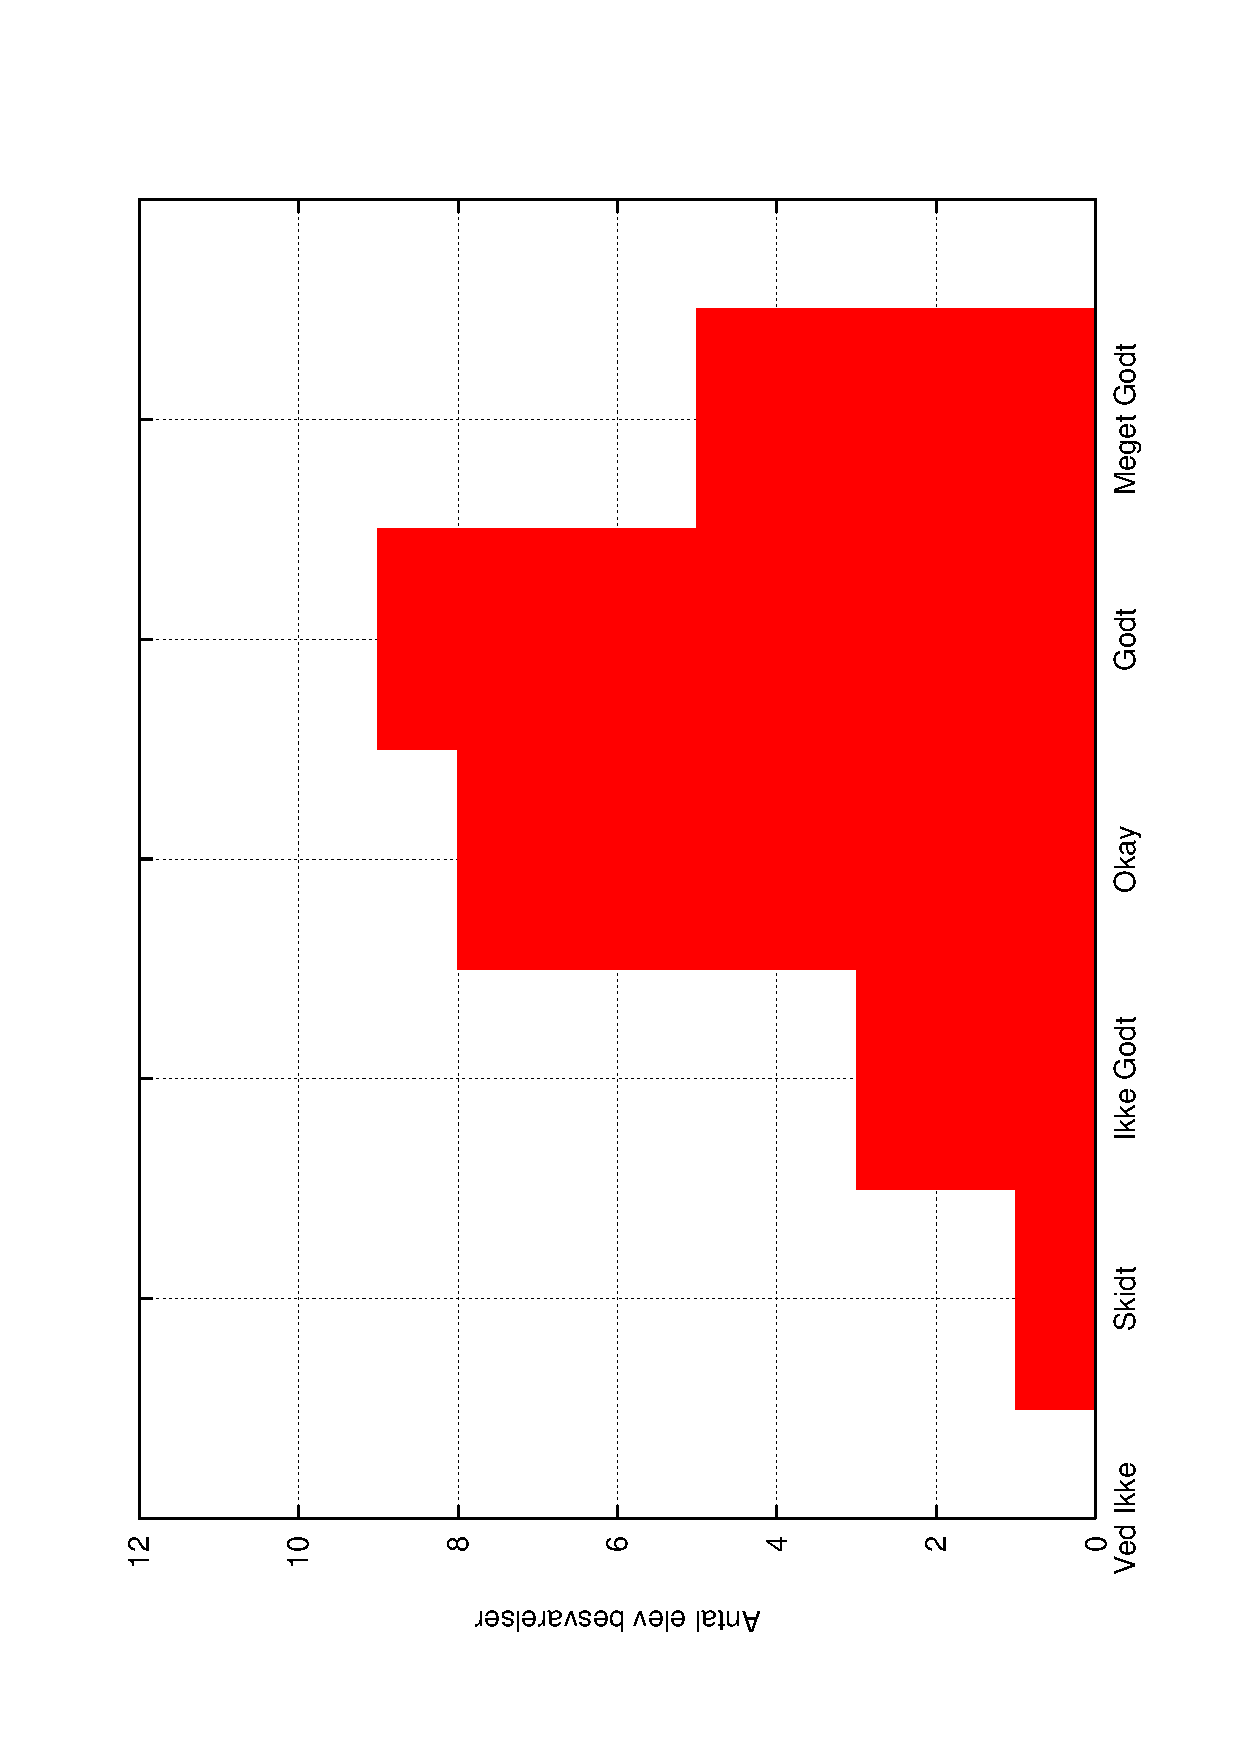
\includegraphics[width=5cm,angle=-90]{enepar}
		\caption{Ene-/pararbejde}
		\label{fig:enepar}
	%\end{figure}
	\vspace{-10pt}
\end{wrapfigure}
Evaluering i 2.bm gav en del datamateriale, da der blev anvendt et lectio sp�rgeskema. Forl�bet var som omtalt i \chapref{DTOF} opbygget om mange forskellige arbejdsformer som aktiverede eleverne og skulle stimulere deres faglige progression. Derfor har eleverne skulle evaluere arbejdsformerne hver for sig. P� en fem trins skala; \emph{skidt, ikke godt, okay, godt og meget godt}. Af denne evaluering ser vi p� \figref{enepar} at eleverne syntes middel godt om arbejdsformen hvor de individuelt skulle besvare nogle studiesp�rgsm�l og efterf�lgende i par skulle diskutere deres svar og med deres f�lles viden svare p� nogle sv�re studiesp�rgsm�l. Noget bedre gik det for arbejdet i grupper og matrixgrupper, som det fremg�r af \figref{gruppe} og \figref{matrix}. Sp�rger man dem om plenum undervisning og klassisk tavleundervisning s� er svaret igen overvejene godt jf. \figref{tavle}, og af \figref{type} fremg�r det at man i 2.bm er s�rdeles glade for at arbejde i grupper b�de konventionelt gruppe arbejde men ogs� matrix grupper. Det eleverne bedst kan lide er dog tavleundervisning hvilket er overraskende n�r eleverne mente at forl�bet indeholdt for meget tavle undervisning. 

\section{~Reflektioner om forl�bet i 2.bm}
\begin{wrapfigure}{l}{7.5cm}
	\vspace{-10pt}
	\centering
	%\begin{figure}[h!]
		%\centering
		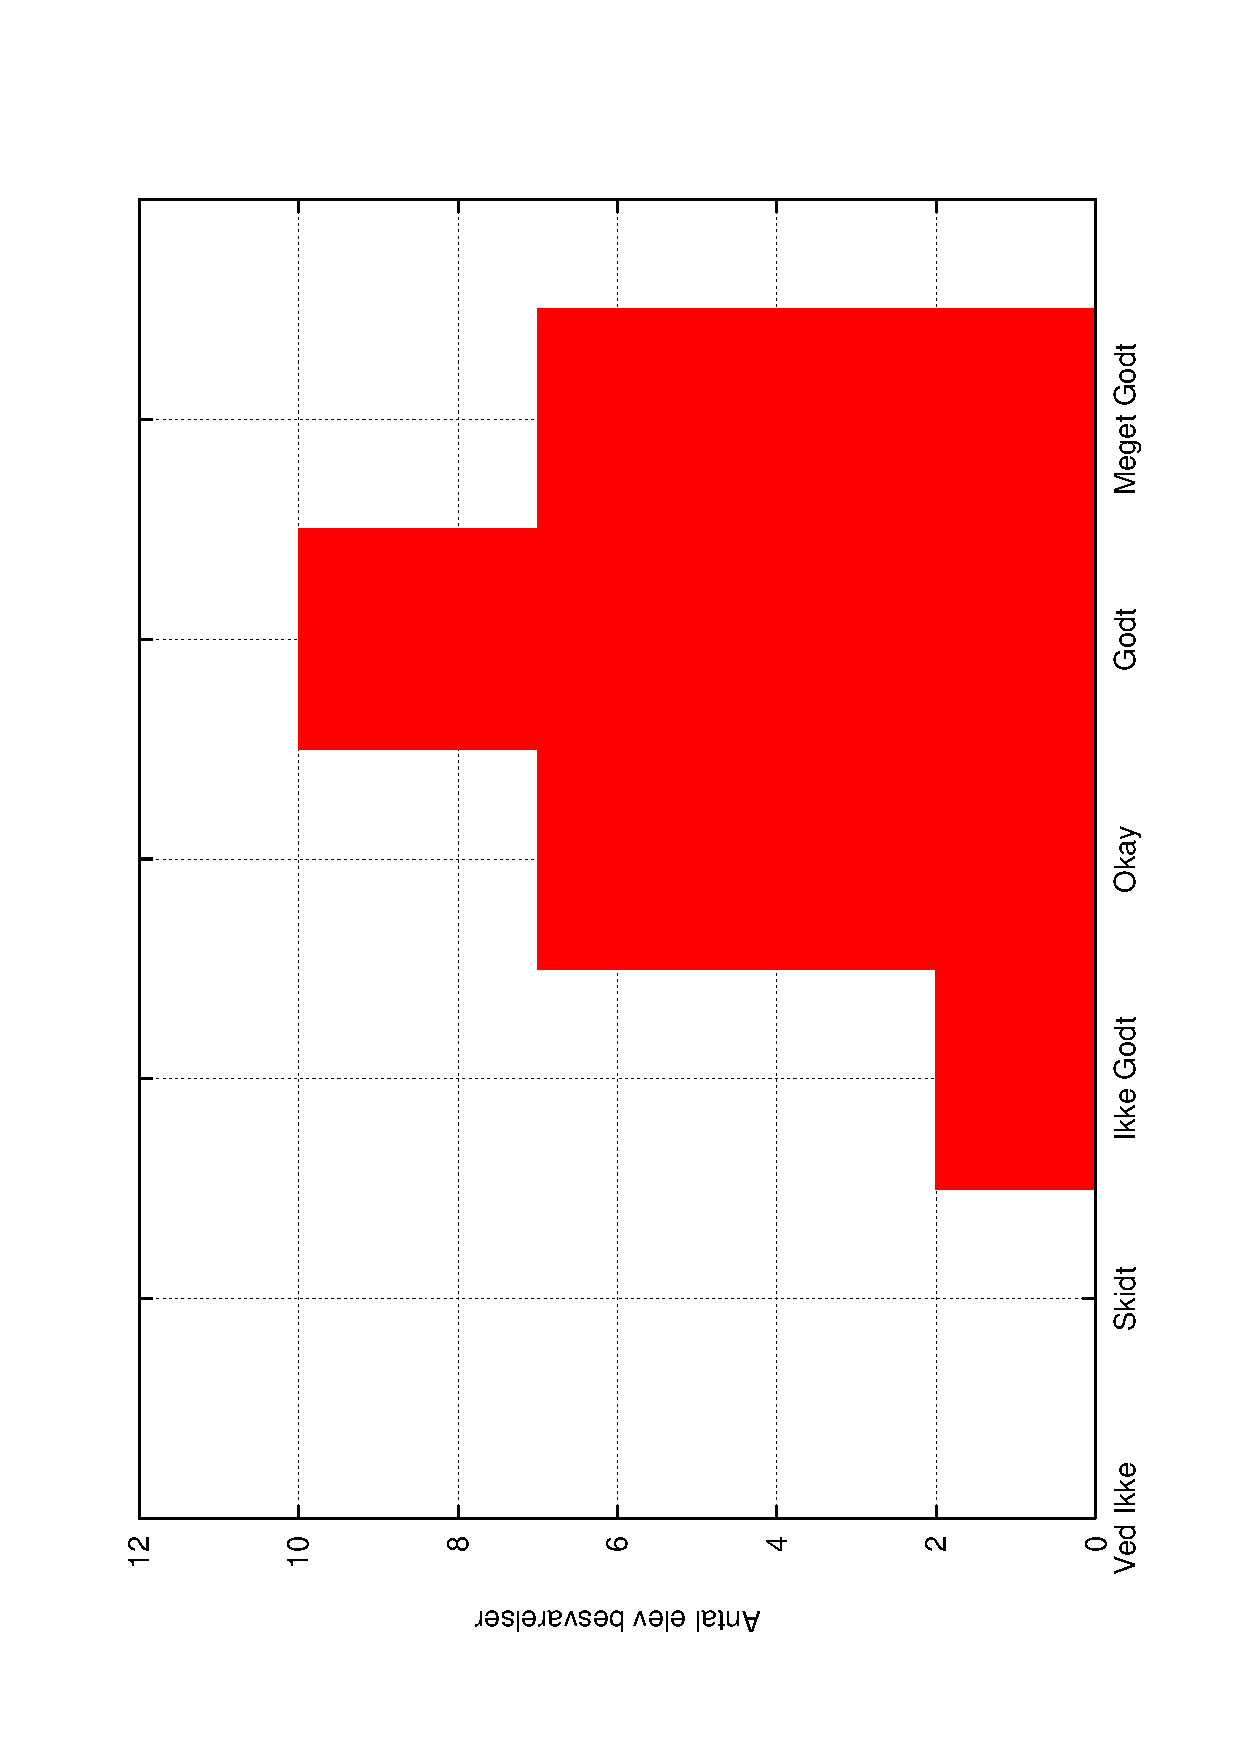
\includegraphics[width=5cm,angle=-90]{gruppe}
		\caption{Gruppearbejde}
		\label{fig:gruppe}
	%\end{figure}
	\vspace{-10pt}
\end{wrapfigure}
Generelt gik forl�bet rigtig godt set med mine �jne, emnet verdensbilleder var ideelt til at arbejde med elevaktiverende undervisningsformer. Dette skyldes at det faglige stof i dette forl�b er p� et niveau hvor eleverne selv er i stand til at tr�kke de vigtigste elementer ud, men samtidig kan stoffet skaleres ved at inddrage relevante kilder dermed g�r vi fra at v�re u uvidende til at blive vidende. Det er min vurdering at Eleverne havde stor udbytte af gruppearbejdet, da de skulle freml�gge for hinanden og havde  et produkt at freml�gge. Ene/par arbejdet var den n�ste arbejdsform som blev testet for at tilgodese de introverte elever. Her var det mit klare indtryk at eleverne fik rigtig meget ud af det. Der var dog et par  frustrationer med hvordan de skulle gribe opgaven an. Dog har de ekstroverte elever som har behov for at �tale for at t�nke� de har det sv�rt med denne arbejdsform hvor de f�rst skal t�nke over en r�kke svar og derved ikke har mulighed for at tale med hinanden. 

\begin{wrapfigure}{r}{7.5cm}
	\vspace{-10pt}
	\centering
	%\begin{figure}[h!]
		%\centering
		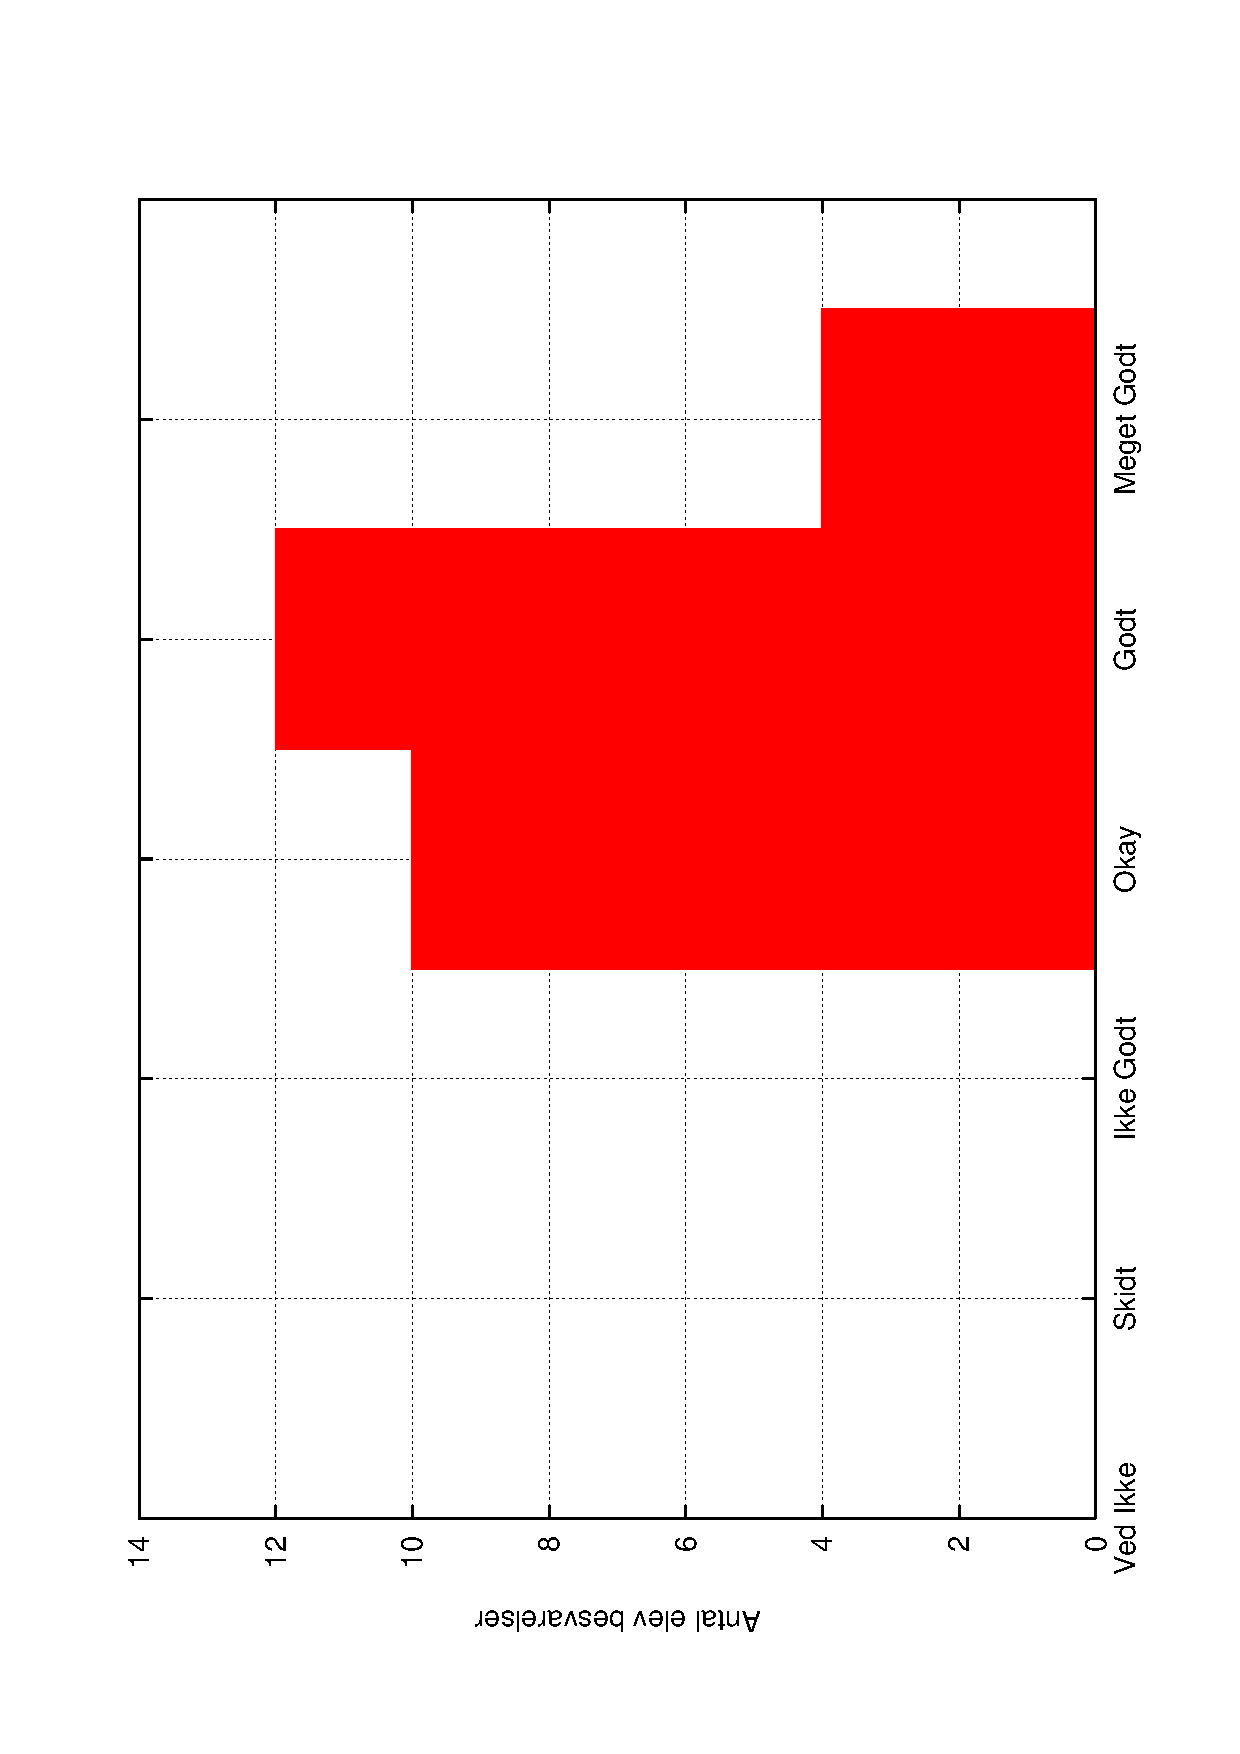
\includegraphics[width=5cm,angle=-90]{matrix}
		\caption{Arbejde i matrix grupper}
		\label{fig:matrix}
	%\end{figure}
	\vspace{-10pt}
\end{wrapfigure}
Sluttelig havde vi et stort anlagt arbejde i matrix-grupper som eleverne vurderede til at v�re meget godt. Her ser vi at eleverne udelukkende er positive. 
Det er tydeligvis det som eleverne finder bedst for deres indl�ring, dette ligger ogs� i god tr�d med at de kommer igennem tingene flere gange b�de gennem et l�rerstyrret intro opl�g og herefter intenst 60 min gruppearbejde, hvor de skal give hinanden lektier for, efterf�lgende skal de pr�sentere deres lektier for deres gruppe hvorefter der formes de nye grupper efter matrix princippet. Eleverne skal nu pr�sentere alt hvad den gamle gruppe har fundet ud af. Sp�rger man i stedet eleverne hvad deres udbytte var af tavle opl�gene er de meget store tilh�ngere af tavleundervisning. Der er med andre ord ikke behov for store �ndringer i forl�bet for at sikre at eleverne flyttes fagligt. 


\section{~Skal praksis �ndres?}
\begin{wrapfigure}{c}{7.5cm}
	\vspace{-10pt}
	\centering
	%\begin{figure}[h!]
		%\centering
		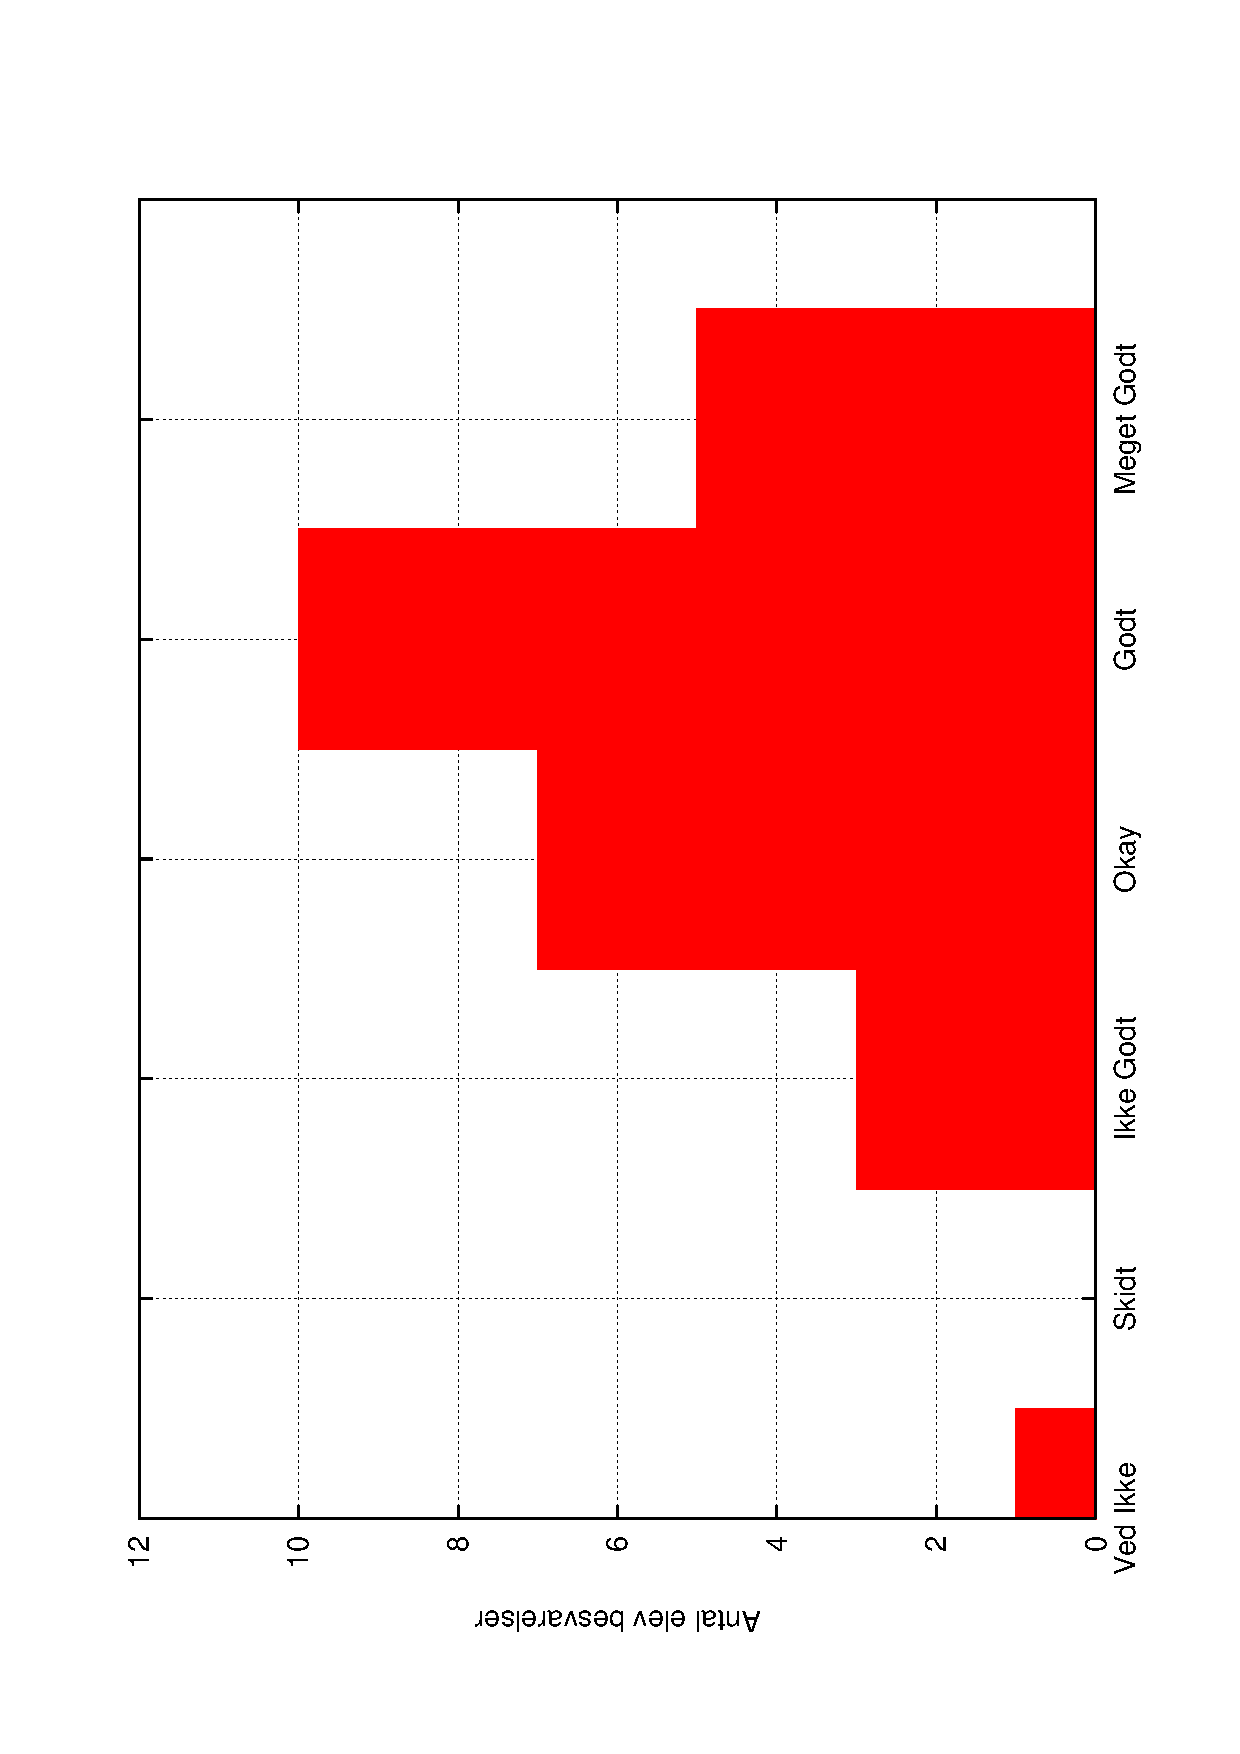
\includegraphics[width=5cm,angle=-90]{tavle}
		\caption{L�restyrret undervisning / Tavle undervisning}
		\label{fig:tavle}
	%\end{figure}
	\vspace{-10pt}
\end{wrapfigure}
Der er nogle ting som ikke virker i 2.bm som klasse f.eks. er klassen ikke s� begejstret for arbejdet med for meget tavle undervisning til trods for at vi kun har haft ca 120 min tavleundervisning fordelt p� 9 moduler svarende til ca 15 \% af undervisnings tiden dermed er knap 85 \% af tiden g�et med elevaktiviteter. Der var flere elever som p�egede at de ikke har behov for reflektions tid for dem selv f�r man g�r til par eller gruppe arbejde. 
Jeg er dog af den opfattelse at de f�r et st�rre udbytte hvis de er klar over deres egne holdninger f�r de kommer til et emne hvor de skal diskutere deres forst�else og holdninger til en problemstilling med andre.
\section{~Evaluering af forl�bet i 1.m}
\begin{wrapfigure}{r}{7.5cm}
	\vspace{-10pt}
	\centering
	%\begin{figure}[h!]
		%\centering
		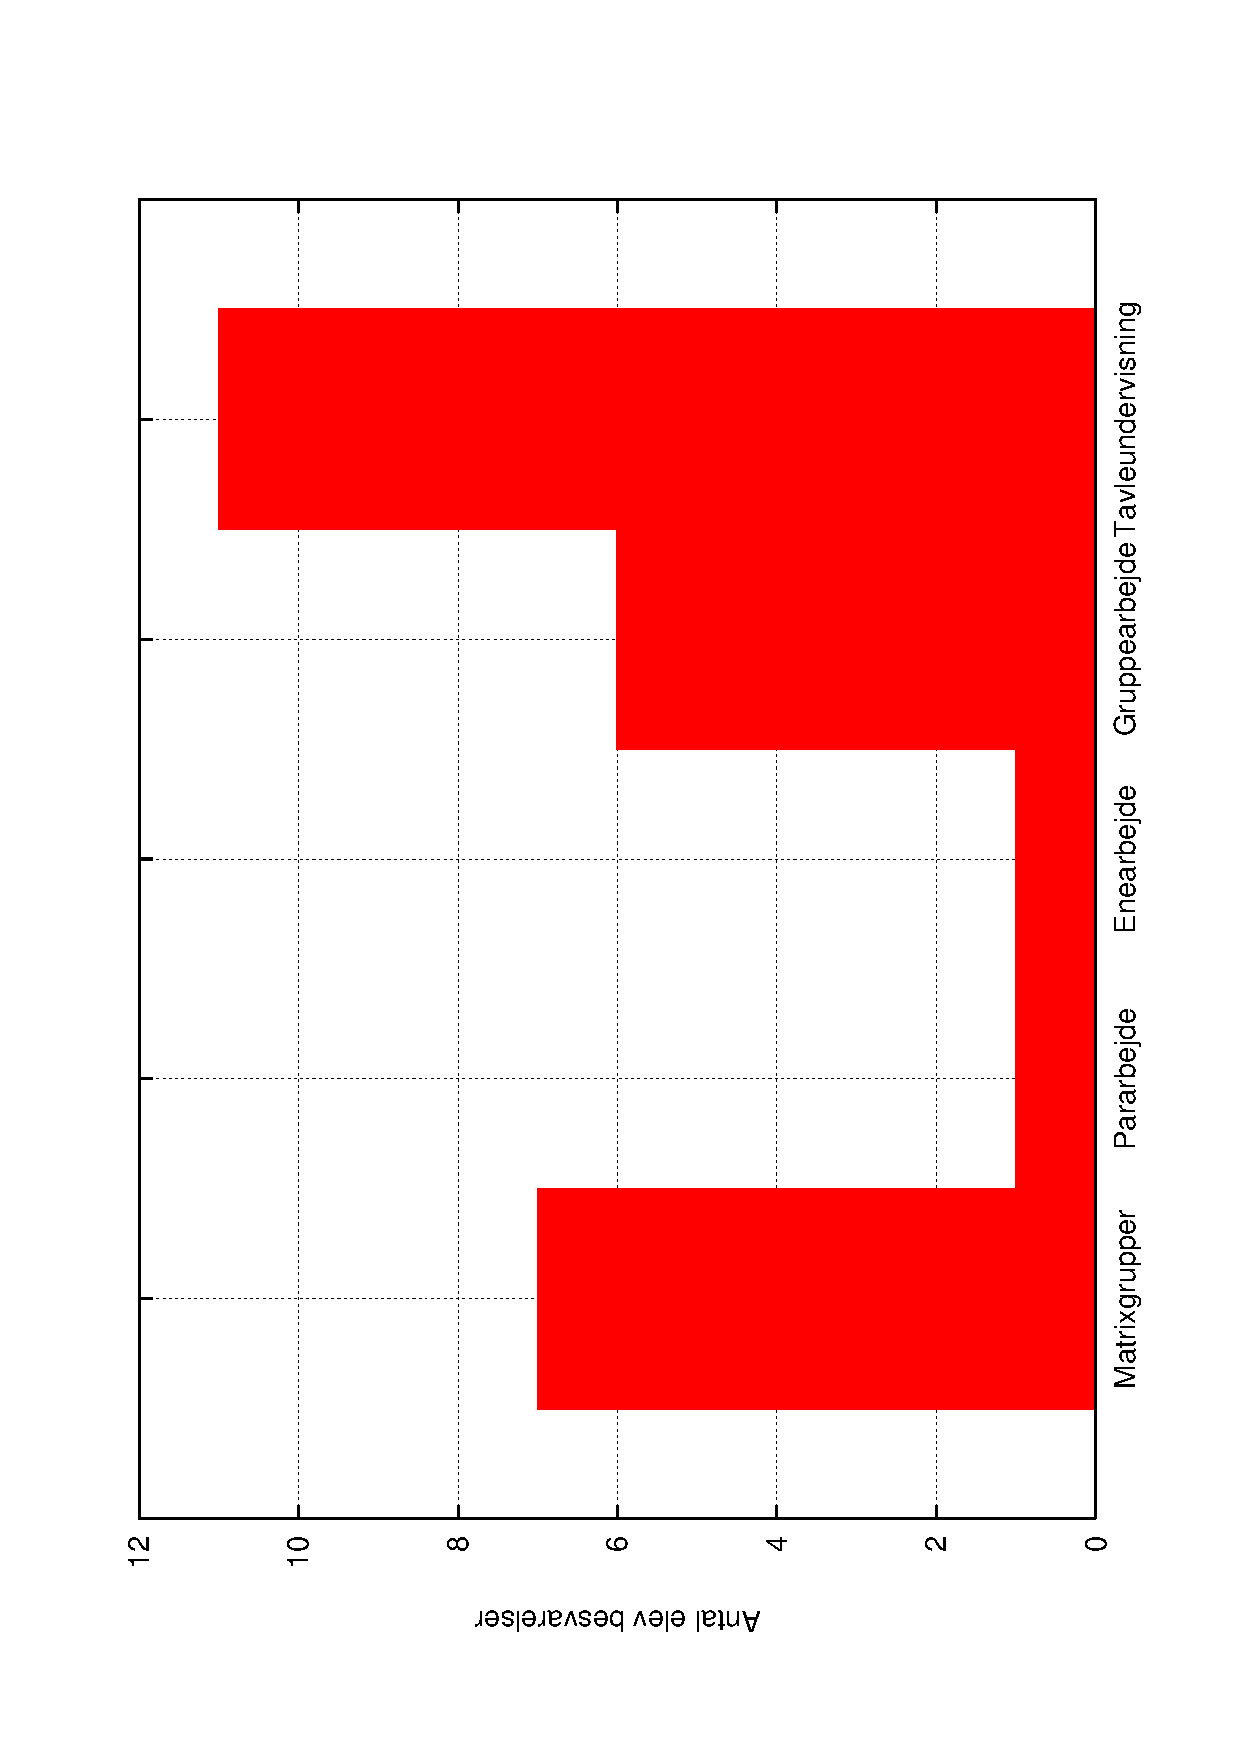
\includegraphics[width=5cm,angle=-90]{type}
		\caption{Foretrukket undervisnings type}
		\label{fig:type}
	%\end{figure}
	\vspace{-10pt}
\end{wrapfigure}
Forl�bet verdensbilleder har I �r fyldt meget i undervisningen for hhv. 2.bm og 1.m forl�bet blev f�rst afpr�vet i 2.bm og efterf�lgende rettet lidt til inden det blev brugt i 1.m. Forl�bet er en gennemgang af den videnskabsteoretiske del af fysik undervisningen. Det er mit indtryk at mange undervisere i fysik overser betydningen af dette forl�b. Derfor har jeg i �r valgt at forl�bet skal give en dyb forst�else af nogle af de paradigmeskift som har f�rt til det verdensbillede vi har idag. Forl�bet er blevet gennemf�rt med udgangspunkt i nogle af de naturvidenskabelige skikkelser som har domineret og udfordret verdensbilledet. Forl�bet tog sit afs�t i Aristoteles og tanken om de fire elementer og byggede liges� stille op til det verdensbillede vi kender. Undervejs i undervisningen har f�lgende typer af undervisning v�ret anvendt.
 Sm� quizzer, Gruppearbejde, L�rerstyret gennemgang, plenum diskussioner, Elev-ene arbejde samt elev-par arbejde. Der har v�ret produktkrav involveret i form af freml�ggelser for klassen og gruppearbejde efter matrix princippet. I 1.m sluttede forl�bet med at vi diskuterede det moderne verdensbillede men de fire fundamentale kr�fter, da disse blev introduceret i et afsnit af Danskernes Akademi. I 1.m har vi i stedet for en mundtlig evaluering som den der blev lavet med 2.bm lavet en skriftlig evaluering i form af en rapport hvor i eleverne skulle m�le Solens rotationstid ved at studere solpletter. Resultatet af denne faglige evaluering se \figref{solplet}. Af denne faglige evaluering ses ikke kun at det er en engageret og dygtig klasse men ogs� at klassen udvikler sig, hvis man sammenligner med klassens karaktere fra evaluering af forl�bet energi. Forl�bet virkede i begge klasser efter hensigten og det var i s�rdeleshed godt at indl�gge udsendelsen fra danskernes akademi som gav anledning til en diskussion af det gamle kontra de nye verdensbillede.
\chapter{Opsamling og Konklusion}
\label{ch:konk}

Progression handler i daglig tale om at flytte sig, det kan v�re i form af ny viden som udvider ens egen horisont. Progression i faglighed handler i h�j grad om kompetencer og forst�else for hvis man ikke har forst�et den viden man har l�rt om kan man ikke anvende den, og kan man ikke anvende den forst�r man ikke dens kompleksitet. Som undervisere skal vi flytte eleverne fra et stadie hvor de m�ske er pr�-strukturelle til et niveau hvor de er relationelt t�nkende hvilket vil sige at de g�r fra et 0-niveau til et niveau hvor de kan forbinde og anvende begreber og centrale analyse metoder. Men f�r vi som undervisere kan flytte eleverne, skal de v�re villige til at l�re. Denne villighed fra elevernes side kan kun opst� hvis eleverne f�ler at de bliver taget seri�st og at de bliver udfordret p� deres eget niveau. Derfor er det vigtigt at man som underviser forst�r at optr�de i forskellige roller over for forskellige elever, her kan man g�re brug af de fire l�ringsrum som Beck og Gottlieb pr�senterede i \citep{Beck:2002}, endvidere b�r man lede klassen jf. den situationsbestemte ledelse jf. \citep{Hersey1, Herse2}. N�r f�rst eleverne er inspirerede handler det om at give dem muligheder for at f� den personlige oplevelse og give dem det rum der g�r de kan reflektere over deres egen oplevelse derved skabe det fundament som Dewey beskriver giver anledning til l�ring.  Herved vil eleverne opn� ny viden og dermed ny indsigt som vil �bne faget for dem. Dette er kernen i den faglige progression. Den faglige progression opst�r alts� allerede i underviserens forberedelse af det enkelte forl�b, hvor underviseren g�r sig tanker om undervisningsformer, arbejdsstof, og hvor selve undervisningens tilrettel�ggelse. Men ogs� empati og evnen til at fornemme hvor eleverne er er en naturlig del af det at skabe god progression for eleverne.

Gennem denne opgave har jeg s�gt at motivere at eleverne gennem klasserums ledelse, omend ledelsen foreg�r i tilrettel�ggelsen af undervisningen \citep{EVA:2013, Meyer:2008, leder:2010, Alstrup:1997, DDS:2006, Hersey1, Herse2}.  Eller i selve afviklingen af en given aktivitet s� er det alfa omega at man som underviser hj�lper eleverne til at opn� den personlige oplevelse som kan starte en l�rings process om man s� er mere eller mindre styret af den l�replan man er underlagt s� er det altid underviserens ansvar at br�nde igennem til eleverne gennem sp�ndende og n�rv�rende undervisning.

Vi kan alts� konkludere at den faglige progression er et samspil mellem mange elementer, f.eks hvordan man i sin forberedelse sikre elevernes faglige progression denne kan v�re dikteret af l�replanen eller den kan v�re mere op til den enkelte underviser, I faget fysik er vi bundet af fagets l�replan, og faget har dermed en naturlig progression indbygget i den m�de kerne stoffet er struktureret p�. Det er dog �nskv�rdigt at indbygge yderligere progression i sine forl�b hvor vi gennem valg af planl�gningsv�rkt�jer kan optimere vores process, og sikre progression for mange elevgrupper p� en gang. Her er v�rkt�jer som FIMME modellen, den didaktiske relationsmodel og 4MAT\textregistered, oplagte v�rkt�jer som vil g�re livet lettere for os som undervisere. Sluttelig er der selve afviklingen hvor vi som undervisere st�r p� m�l for den tilrettelagte progression i faget. Her skal vi hele tiden tilpasse planer og niveau efter forholdene og eleverne, s�ledes at elverne f�r bygget det h�jest mulige korthus. Dermed er vi alts� ogs� n�dt til at hj�lpe forskellige elever p� forskellige m�der. Her er det efter min over bedste overbevisning vigtigt at have kendskab til personlighedstypologi, jf. \citep{MBTI, JTI,jung1923psychological, DDS:2006, Alstrup:1997, Ringstad:2002} samt ledelse af forskellige individer p� forskellig m�de jf. \citep{Hersey1, Herse2, Alstrup:1997, DDS:2006}.  Det er alts� muligt for en underviser at sikre den enkelte elevs faglige progression i klasserummet, gennem fornuftig ledelse.\vspace{.5cm}
\begin{flushright}
Thomas Mellergaard Amby
\end{flushright}


\begin{appendix}
\chapter[Undervisnings forl�bet Verdensbilleder]{Verdensbilleder}
\label{app:Verden}
\section{~Form�l:}
Form�let med forl�bet om fysikkens bidrag til verdensbilleders udvikling, er at give eleverne en forst�else af at fysikken har bidraget til at udvikle dem m�de vi opfatter den verden vi lever i. Gennem eksperimenter og teoretiske betragtninger skal vi se p� hvorledes verden har �ndret sig fra Ptolemaios og frem til vore dages s�gen efter exoplaneter.

\section{~Indhold:}
Forl�bet vil v�re bygget op hhv. omkring stoffet i FysikABbogen 1�s kapitel 3 om verdensbilledet, men i liges� stor grad p� noter som vil blive udleveret i forbindelse med undervisningen. Disse noter vil v�re skrevet og tilrettelagt s�ledes at de bygger videre p� de kerne tekster som ligger i kapitlet fra Benoni et al. Forl�bet er t�nkt s� det f�lger en naturlig r�dtr�d gennem de �rstal som vi skal dykke ned i. Forl�bet t�nkes at l�be over 10 moduler af  90 min.

\section{~Metode:}
Metoden som t�nkes anvendt her, er hhv. eksperimentel da det er vigtigt for eleverne at l�re at s�tte ind i hvorledes man t�nkte i oldtiden, samt i ren�ssancen endda ogs� i nyere tid.  Gennem denne t�nkning vil eleverne ogs� indse hvorfor man har draget de slutninger man har. Andre typer af undervisningsformer som t�nkes anvendt er grupper og matrix grupper da fokus i klassen pt. Er p� elevaktiverende undervisning. Ydermere t�nkes der en teoretisk dimension, hvor vi snuser til meget af den underliggende teori, og i det store hele vil forl�bet tjene som en form or oversigts l�sning i hvilke interessante emner klassen skal igennem i det 2 �rige  B-niveau.

\section{~Materiale:}
Materialet vil som omtalt i afsnittet indhold prim�rt v�re kapitlet i bogen men ogs� noter fra timen vil blive anvendt som en del af undervisningens pensum, her t�nkes specielt p� opl�g til gruppe arbejde.

\section{~Evaluering:}
I forhold til evalueringen af dette forl�b t�nkes der at vi l�bende vil evaluere processen gennem sm� interaktive quizzer med programmet socrative (\href{http://m.socrative.com}{m.socrative.com}). Dette vil give os et direkte m�l for elevernes progression gennem forl�bet. Endvidere t�nkes det at eleverne skal skrive en rapport om nogle af de ting der er arbejdet med, for at give et helheds billeder af om eleverne har forst�et stoffet. 

\section{~Modul plan:}


\begin{table}
	\centering
	\caption[Verdensbilleder - Modul 1 -- Mit eget verdensbillede]{Modul 1 - Mit eget verdensbillede}
	\begin{tabular}{@{ } l p{2.5cm} p{4cm} p{5cm} @{ }}
		\toprule[2pt]
		{\bf Tid [min]} & {\bf Aktivitet} & {\bf Beskrivelse af aktivitet} & {\bf Didaktiske overvejelser}\\
		\midrule
		0 & Pr�sentation af dagens program & Kort skematisk pr�sentation af den film som skal ses & Dette g�res for at eleverne er bekendte med at der vil komme en opgave som forholder sig til filmen � og at der derfor kan v�re en ide at tage noter. \\
		\midrule
		3 & Se film & Vi ser filmen: Danskernes Akademi � Verdens st�rste fysikeksperiment  & At give eleverne en ny type indsigt i den verden de selv lever i.\\
		\midrule
		80 & Der samles op p� dagens afsnit af filmen & Vi n�r ikke at se hele filmen derfor samler vi kort op p� hvad vi har f�et at vide i dag, inden der rydes op og lokalet forlades & S�rg for at Eleverne tager noget med sig fra timen.\\
		\bottomrule[2pt]
	\end{tabular}
\end{table}


\begin{table}
	\centering
	\caption[Verdensbilleder - Modul 2 -- Mit eget verdensbillede del 2]{Modul 2 - Mit eget verdensbillede del 2}
	\begin{tabular}{@{ } l p{2.5cm} p{4cm} p{5cm} @{ }}
		\toprule[2pt]
		{\bf Tid [min]} & {\bf Aktivitet} & {\bf Beskrivelse af aktivitet} & {\bf Didaktiske overvejelser}\\
		\midrule
		0 & Pr�sentation af dagens program & Kort skematisk pr�sentation af den film som skal ses & Dette g�res for at eleverne er bekendte med at der vil komme en opgave som forholder sig til filmen � og at der derfor kan v�re en ide at tage noter. \\
		\midrule
		3 & Se film - fortsat & Vi ser filmen: Danskernes Akademi � Verdens st�rste fysikeksperiment  & At give eleverne en ny type indsigt i den verden de selv lever i.\\
		\midrule
		45 & Beskriv dit verdenssyn & Med udgangspunkt i filmen om CERN og LHC skal eleverne beskrive den verden de selv lever i og hvad konsekvensen for den almindelige dansker er. & Opgaven tvinger eleverne til at fundere over den verden de lever i og hvordan de opfatter den\\
		\midrule
		75 & Diskussion af verdensbilledet i dag plenum & Med udgangspkt. I en eller flere af elevernes beskrivelser af verdensbilledet i dag snakker vi om betydningen for den almene dansker & Diskussionen foreg�r i Plenum, men den forudg�ende skriftlige �velse sikre at alle har noget at byde ind med og at alle har gjort sig nogle overvejelser\\
		\midrule
		85 & Der ryddes op & Lokalet skal forlades p�nt og ordentligt & Tak for idag\ldots\\
		\bottomrule[2pt]
	\end{tabular}
\end{table}

\begin{table}
	\centering
	\caption[Verdensbilleder - Modul 3 -- Fra Aristoteles til Kopernikus]{Modul 3 - Fra Aristoteles til Kopernikus}
	\begin{tabular}{@{ } l p{2.5cm} p{4cm} p{5cm} @{ }}
		\toprule[2pt]
		{\bf Tid [min]} & {\bf Aktivitet} & {\bf Beskrivelse af aktivitet} & {\bf Didaktiske overvejelser}\\
		\midrule
		0 & Opsamling fra sidst & Kort opsummering af timen ig�r, Disse skal kort gennemg�es af eleverne p� tavlen. & Dette g�res for at sikre at alle har forst�et hvorledes verden i dag h�nger sammen\\
		\midrule
		10 & Pr�sentation af det nye emne � Mindmap p� tavlen. & Associativ �velse, �velsens form�l er at f� eleverne tili f�llesskab at finde ud af hvad et verdensbillede egentlig er og hvordan fysikken kan bidrage.  & Dette bliver totalt kaos, men vil give os en ide om elevernes forh�ndsforst�else for forl�bets indhold.\\
		\midrule
		30 & Pr�sentation af dagens n�gle personer. & Personerne som vi skal arbejde med skal pr�senteres  s�ledes at alle ved hvad hvem vi skal arbejde med og hvorledes de opfattede verden.  & At give eleverne et f�lles forforst�else for dagens arbejde i grupper.\\
		\midrule
		60 & Gruppe arbejde & Klassen deles i 6 grupper: tre grupper besk�ftiger sig med hvilke personer vi har i spil: Aristoteles, Ptolemaios og Kopernikus. 3 grupper laver eksperimenter, som man ville have gjort p� deres tid. Produktet skal v�re en 5 min. Pr�sentation for resten af klassen omhandlende resultater og/eller hvem personen var. &  Her gives resten af timen til fordybende arbejde. Med de tre kerne personer\\
		\midrule
		85 & Der rydes op & Lokalet skal forlades p�nt og ordenligt. & Hvordan var timens forl�b?
Feedback fra: Ahmed, Arina \& Casper Juul\\
		\bottomrule[2pt]
	\end{tabular}
\end{table}

\begin{table}
	\centering
	\caption[Verdensbilleder - Modul 4 -- Fra Kopernikus til Newton]{Modul 4 - Fra Kopernikus til Newton}
	\begin{tabular}{@{ } l p{2.5cm} p{4cm} p{5cm} @{ }}
		\toprule[2pt]
		{\bf Tid [min]} & {\bf Aktivitet} & {\bf Beskrivelse af aktivitet} & {\bf Didaktiske overvejelser}\\
		\midrule
		0 & Opsamling fra sidst & Vi gennemg�r de opgaver som grupperne havde sidst, hver gruppe m� max have 2 slides. & �velse I kort at pr�sentere udvalgt stof for en given m�lgruppe samt at vidensdele indternt (og p� FC)\\
		\midrule
		40 & Pr�sentation af dagens n�gle personer. & Personerne som vi skal arbejde med skal pr�senteres  s�ledes at alle ved hvad hvem vi skal arbejde med og hvorledes de opfattede verden. & Kernen her vil ligge i hvorledes verden s� ud inden Newton og hvilke landvindinger der var sket mellem antikken og s� frem til Gallilei. \\
		\midrule
		60 & Opl�g til par arbejde & Der give instrukser til hvorledes der skal arbejde resten af timen. & Dagens anden store elev aktivering vil ligge i form af et par arbejde. Her vil v�re nogle sp�rgsm�l som vil har deres udgangspunkt i den l�ste tekst. Samt nogle hvortil informations s�gning p� nettet vil v�re n�dvendig.\\
		\midrule
		85 & Der rydes op & Lokalet skal forlades p�nt og ordenligt.resultater og/eller hvem personen var. & Hvordan forl�b timen?
Feedback fra:
Casper O., Christian S. \& Gerd\\
		\bottomrule[2pt]
	\end{tabular}
\end{table}

\begin{table}
	\centering
	\caption[Verdensbilleder - Modul 5 -- Verden efter Newton]{Modul 5 - Verden efter Newton}
	\begin{tabular}{@{ } l p{2.5cm} p{4cm} p{5cm} @{ }}
		\toprule[2pt]
		{\bf Tid [min]} & {\bf Aktivitet} & {\bf Beskrivelse af aktivitet} & {\bf Didaktiske overvejelser}\\
		\midrule
		0 & Opsamling fra sidst & Vi gennemg�r det par arbejde som blev lavet sidst. & Her er �velsen at eleverne nu i lidt st�rrer grupper sammen gennemg�r det der blev lavet sidst.\\
		\midrule
		20 & Fra Newton til Hubble & Personerne som vi skal arbejde med skal pr�senteres  s�ledes at alle ved hvad hvem vi skal arbejde med og hvorledes de opfattede verden. & Kernen her vil ligge i hvorledes verden s� ud inden Newton og hvilke landvindinger der var sket mellem antikken og s� frem til Gallilei. \\
		\midrule
		60 & Gruppe arbejde om en r�kke opgaver. & Der regnes opgaver  & Hj�lpe med elevernes forst�else af stoffet.\\
		\midrule
		85 & Der rydes op & Lokalet skal forlades p�nt og ordenligt.resultater og/eller hvem personen var. & Hvordan forl�b timen?
Feedback fra:
Hamza, Hjalte \&Jakob\\
		\bottomrule[2pt]
	\end{tabular}
\end{table}

\begin{table}
	\centering
	\caption[Verdensbilleder - Modul 6 -- P� opdagelse i solsystemet]{Modul 6 - P� opdagelse i solsystemet}
	\begin{tabular}{@{ } l p{2.5cm} p{4cm} p{5cm} @{ }}
		\toprule[2pt]
		{\bf Tid [min]} & {\bf Aktivitet} & {\bf Beskrivelse af aktivitet} & {\bf Didaktiske overvejelser}\\
		\midrule
		0 & Opsamling fra sidst & Der samles kort op p� det arbejde som er blevet lavet frem til og med Hubble. Dermed �bner vi d�ren til astronomien & Plenums diskussion af hvordan verdensbilledet har udviklet sig siden Aristoteles. \\
		\midrule
		15 & Opl�g om solsystemets dannelse.  & Slide show gennemgang af solsystemets dannelse & H�j l�re styring for at sikre at alle har minimum en smal for-forst�else for dette emne inden gruppe arbejdet indledes\\
		\midrule
		45 & Del et af gruppe arbejde om solsystemet & Hver gruppe f�r en arbejdsseddel med sp�rgsm�l og ting som gruppen skal unders�ge. Ydermere skal gruppen give hinanden lektier for. & Opgaven er at eleverne selv fordyber sig i stoffet. Og bidrager til deres f�lles forst�else af stoffet\\
		\midrule
		85 & Der rydes op & Lokalet skal forlades p�nt og ordenligt.resultater og/eller hvem personen var. & Hvordan forl�b timen?
Feedback fra:
Jamie, Jeppe \& Jonas\\
		\bottomrule[2pt]
	\end{tabular}
\end{table}

\begin{table}
	\centering
	\caption[Verdensbilleder - Modul 7 -- P� opdagelse i solsystemet del 2]{Modul 7 - P� opdagelse i solsystemet del 2}
	\begin{tabular}{@{ } l p{2.5cm} p{4cm} p{5cm} @{ }}
		\toprule[2pt]
		{\bf Tid [min]} & {\bf Aktivitet} & {\bf Beskrivelse af aktivitet} & {\bf Didaktiske overvejelser}\\
		\midrule
		0 & 	Opsamling fra sidst & Grupperne fra sidst diskutere deres lektier s�ledes at de har en st�rre viden at tage med i matrix arbejdet. & �velsen her er at eleverne �ver sig i at formidle en specifik viden som kun de ligger inde med. (under tidspres)\\
		\midrule
		30 & MATRIX & Der formes nye grupper efter matrix princippet og der formidles nu med udgangspunkt i det som de indledende grupper havde haft som emne & Eleverne skulle nu opn� en mere generel forst�else af solsystemet og dets komponenter og spidsfindigheder.\\
		\midrule
		85 & Der rydes op & Lokalet skal forlades p�nt og ordenligt.resultater og/eller hvem personen var. & Hvordan forl�b timen?
Feedback fra:
Josephine, Kathrine\& Kristian\\
		\bottomrule[2pt]
	\end{tabular}
\end{table}

\begin{table}
	\centering
	\caption[Verdensbilleder - Modul 8 -- Jagten p� liv]{Modul 8 - Jagten p� liv}
	\begin{tabular}{@{ } l p{2.5cm} p{4cm} p{5cm} @{ }}
		\toprule[2pt]
		{\bf Tid [min]} & {\bf Aktivitet} & {\bf Beskrivelse af aktivitet} & {\bf Didaktiske overvejelser}\\
		\midrule
		0 & Opsamling fra sidst & Der samles op p� hvad vi har l�rt om solsystemet og de andre ting som har p�virket det verdensbillede vi har idag. & Dette g�res for at give eleverne overblik samt for at genopfriske detaljer.\\
		\midrule
		20 & Betydning af verdensbilledet  & Hvilken betydning har verdensbilledet for den forskning vi foretager i dag mhp. At finde liv andre steder end p� Jorden. & H�j l�rer styrring � pr�sentation af frontline data og forskning, med indlagte klasse diskussioner\\
		\midrule
		85 & Der rydes op & Lokalet skal forlades p�nt og ordenligt.resultater og/eller hvem personen var. & Hvordan forl�b timen?
Feedback fra:
Lasse, Louise \& Malale\\
		\bottomrule[2pt]
	\end{tabular}
\end{table}

\begin{table}
	\centering
	\caption[Verdensbilleder - Modul 9 -- Bestemmelse af Solens rotationstid]{Modul 9 - Bestemmelse af Solens rotationstid}
	\begin{tabular}{@{ } l p{2.5cm} p{4cm} p{5cm} @{ }}
		\toprule[2pt]
		{\bf Tid [min]} & {\bf Aktivitet} & {\bf Beskrivelse af aktivitet} & {\bf Didaktiske overvejelser}\\
		\midrule
		0 & Pr�sentation af fors�get & Her snakkes om hvorledes man kan gennemf�re eksperimentet. & Dette g�res for at give eleverne overblik samt for at genopfriske detaljer.\\
		\midrule
		10 & FORS�G  & Eleverne udf�rer eksperimentet p� data fra SOHO satellitten& Her f�r de en indsigt i at selv om man har den nyeste teknologi er der stadig nogle ting som man g�r p� en meget low-tech m�de.\\
		\midrule
		85 & Der rydes op & Lokalet skal forlades p�nt og ordenligt.resultater & Tak for idag\ldots\\
		\bottomrule[2pt]
	\end{tabular}
\end{table}

\begin{table}
	\centering
	\caption[Verdensbilleder - Modul 10 -- Bestemmelse af Solens rotationstid skrivemodul]{Modul 10 - Bestemmelse af Solens rotationstid skrivemodul}
	\begin{tabular}{@{ } l p{2.5cm} p{4cm} p{5cm} @{ }}
		\toprule[2pt]
		{\bf Tid [min]} & {\bf Aktivitet} & {\bf Beskrivelse af aktivitet} & {\bf Didaktiske overvejelser}\\
		\midrule
		0 & Opsamling p� fors�get & Vi diskuterer resultater og metoder & Gennemvejledning skulle slutproduktet gerne v�re af h�jere kvalitet\\
		\midrule
		10 & Skrive tid  & Eleverne f�r modulet til at skrive rapport i og stille sp�rgsm�l hvis de er i tvivl. & Her f�r de en indsigt i at selv om man har den nyeste teknologi er der stadig nogle ting som man g�r p� en meget low-tech m�de.\\
		\midrule
		85 & Der rydes op & Lokalet skal forlades p�nt og ordenligt.resultater & Tak for idag\ldots\\
		\bottomrule[2pt]
	\end{tabular}
\end{table}

\chapter[Evaluering af forl�bet Verdensbilleder]{Evaluering af forl�bet}
\label{app:Evaluering}

\section{~Evaluering af forl�bet verdensbilleder}

%\subsection{Hvad synes du om emnet verdensbilleder?}
\begin{Form}
\ChoiceMenu[radio, name=sp1]{\bf \color{DDS}Hvad synes du om emnet verdensbilleder?\\}{Meget Godt=m, Godt = g, Okay=o, Ikke Godt = I, D�rligt=d, Ved Ikke=v}\vspace{.5cm}

\ChoiceMenu[radio, name=sp2]{\bf \color{DDS}Hvordan har sammenh�ngen v�ret gennem forl�bet?\\}{Meget Godt=m, Godt = g, Okay=o, Ikke Godt = I, D�rligt=d, Ved Ikke=v}\vspace{.5cm}

\section{~Evaluering af timerne}
\ChoiceMenu[radio, name=sp3]{\bf \color{DDS}Hvordan har timerne i forl�bet v�ret?\\}{Meget Godt=m, Godt = g, Okay=o, Ikke Godt = I, D�rligt=d, Ved Ikke=v}\vspace{.5cm}

\ChoiceMenu[radio, name=sp4]{\bf \color{DDS}Hvordan Vurdere du det faglige niveau?\\}{Meget Godt=m, Godt = g, Okay=o, Ikke Godt = I, D�rligt=d, Ved Ikke=v}\vspace{.5cm}

\ChoiceMenu[radio, name=sp5]{\bf \color{DDS}Hvorledes vurdere du m�den stoffet blev formidlet p�?\\}{Meget Godt=m, Godt = g, Okay=o, Ikke Godt = I, D�rligt=d, Ved Ikke=v}\vspace{.5cm}

\ChoiceMenu[radio, name=sp6]{\bf \color{DDS}Hvis du skulle bed�mme Thomas' evne som formidler hvilken karakter skulle han s� have?\\}{12=A, 10 = B, 7=C, 4 = D, 02=E, 00=F, -3 = Fx}\vspace{.5cm}

\TextField[name=sp7]{\bf \color{DDS}Begrund din karakter.}\vspace{1.5cm}

\section{~Evaluering af arbejdsformerne}
Gennem forl�bet har vi l�bende arbejdet p� forskellig vis, her t�nkes der bl.a. p� tavleundervisning, gruppearbejde, enearbejde, pararbejde og matrixgrupper.

\ChoiceMenu[radio, name=sp8]{\bf \color{DDS}Hvordan fungerede gruppearbejdet med produkt krav?\\}{Meget Godt=m, Godt = g, Okay=o, Ikke Godt = I, D�rligt=d, Ved Ikke=v}\vspace{.5cm}

\ChoiceMenu[radio, name=sp9]{\bf \color{DDS}Hvordan vudere du ene-/pararbejdet?\\}{Meget Godt=m, Godt = g, Okay=o, Ikke Godt = I, D�rligt=d, Ved Ikke=v}\vspace{.5cm}

\ChoiceMenu[radio, name=sp10]{\bf \color{DDS}Hvordan var arbejdet med solsystemet i matrix grupper?\\}{Meget Godt=m, Godt = g, Okay=o, Ikke Godt = I, D�rligt=d, Ved Ikke=v}\vspace{.5cm}

\ChoiceMenu[radio, name=sp11]{\bf \color{DDS}Vurder dit udbytte af opl�gene p� tavlen\\}{Meget Godt=m, Godt = g, Okay=o, Ikke Godt = I, D�rligt=d, Ved Ikke=v}\vspace{.5cm}

\ChoiceMenu[radio, name=sp12]{\bf \color{DDS}Hvilken type undervisning vil du mene du har f�et mest ud af?\\}{Tavleundervisning=t, Gruppearbejde = g, Enearbejde=e, Pararbejde = p, Matrixgrupper=m}\vspace{.5cm}


\TextField[name=sp13]{\bf \color{DDS}Begrund dit svar.}\vspace{1.5cm}

\section{~Evaluering af Klassen}
\ChoiceMenu[radio, name=sp14]{\bf \color{DDS}Hvordan vil du vurdere dine klasse kammeraters forberedelse til timerne?\\}{Meget Godt=m, Godt = g, Okay=o, Ikke Godt = I, D�rligt=d, Ved Ikke=v}\vspace{.5cm}

\ChoiceMenu[radio, name=sp15]{\bf \color{DDS}Hvordan vurdere du deres indsats i timerne?\\}{Meget Godt=m, Godt = g, Okay=o, Ikke Godt = I, D�rligt=d, Ved Ikke=v}\vspace{.5cm}

\ChoiceMenu[radio, name=sp16]{\bf \color{DDS}Hvis du skulle give klassen som helhed en karakter for deres indstats i forl�bet?\\}{12=A, 10 = B, 7=C, 4 = D, 02=E, 00=F, -3 = Fx}\vspace{.5cm}

\TextField[name=sp17]{\bf \color{DDS}Begrund karakteren.}\vspace{1.5cm}

\ChoiceMenu[radio, name=sp18]{\bf \color{DDS}Hvordan vil du vurdere din egen forberedelse?\\}{Meget Godt=m, Godt = g, Okay=o, Ikke Godt = I, D�rligt=d, Ved Ikke=v}\vspace{.5cm}

\ChoiceMenu[radio, name=sp19]{\bf \color{DDS}Hvordan vil du vurdere din egen indsats i timerne?\\}{Meget Godt=m, Godt = g, Okay=o, Ikke Godt = I, D�rligt=d, Ved Ikke=v}\vspace{.5cm}

\ChoiceMenu[radio, name=sp20]{\bf \color{DDS}Hvor mange timer har du i snit brugt om ugen p� forberedelse til fysik?\\}{0 - 2 timer=a, 2 - 4 timer = b, 4 - 6 timer=c, 6 - 8 timer = d, 8 - 10 timer=e}\vspace{.5cm}

\ChoiceMenu[radio, name=sp21]{\bf \color{DDS}Hvor lang tid mener du man burde bruge p� forberedelse til fysik?\\}{0 - 2 timer=a, 2 - 4 timer = b, 4 - 6 timer=c, 6 - 8 timer = d, 8 - 10 timer=e}\vspace{.5cm}

\ChoiceMenu[radio, name=sp22]{\bf \color{DDS}Hvis du skulle give dig selv en karakter p� baggrund af din indsats?\\}{12=A, 10 = B, 7=C, 4 = D, 02=E, 00=F, -3 = Fx}\vspace{.5cm}

\TextField[name=sp23]{\bf \color{DDS}Begrund dit valg af karakter.}\vspace{1.5cm}

\section{~Forbedringer}

\TextField[name=sp24]{\bf \color{DDS}Hvad var godt? (N�vn 3 ting som var gode)}\vspace{1.5cm}

\TextField[name=sp25]{\bf \color{DDS}Hvad kan g�res bedre? (N�vn 3 ting som kunne g�res bedre)}\vspace{1.5cm}

\TextField[name=sp26]{\bf \color{DDS}Hvordan kunne forl�bet g�res endnu bedre? (Hvis vi nu skulle �ndre p� en ting for at det hele bliver meget bedre, hvad skulle s� �ndres?}\vspace{1.5cm}
\end{Form}

\end{appendix}

\backmatter
%\begin{thebibliography}{}
\bibliography{bibliografi/bibliografi}
%\end{thebibliography}

\end{document}